
%========= File containing the main LaTex document ========%
%                                                          %
% Copyright (C) ISI - All Rights Reserved                  %
% Proprietary                                              %
% Written by Med Hossam <med.hossam@gmail.com>, April 2016 %
%                                                          %
% @author: HEDHILI Med Houssemeddine                       %
% @linkedin: http://tn.linkedin.com/in/medhossam           %
%==========================================================%

%\documentclass[pfe]{./tpl/isipfe}
\documentclass[]{./tpl/isipfe}
\graphicspath{{./img/}}

%\usepackage{hyperref}


\newenvironment{changemargin}[2]{%
\begin{list}{}{%
\setlength{\leftmargin}{#1}%
\setlength{\rightmargin}{#2}%
}%
\item[]}
{\end{list}}

\makeatletter

%================= front cover variables =================%

\newcommand{\secondAuthor}[1]{\gdef\@secondAuthor{#1}}%
\newcommand{\@secondAuthor}{\@latex@warning@no@line{No \noexpand\secondAuthor given}}

\newcommand{\diplomaName}[1]{\gdef\@diplomaName{#1}}%
\newcommand{\@diplomaName}{\@latex@warning@no@line{No \noexpand\diplomaName given}}

\newcommand{\speciality}[1]{\gdef\@speciality{#1}}%
\newcommand{\@speciality}{\@latex@warning@no@line{No \noexpand\speciality given}}

\newcommand{\proFramerName}[1]{\gdef\@proFramerName{#1}}%
\newcommand{\@proFramerName}{\@latex@warning@no@line{No \noexpand\proFramerName given}}

\newcommand{\proFramerSpeciality}[1]{\gdef\@proFramerSpeciality{#1}}%
\newcommand{\@proFramerSpeciality}{\@latex@warning@no@line{No \noexpand\proFramerSpeciality given}}

\newcommand{\academicFramerName}[1]{\gdef\@academicFramerName{#1}}%
\newcommand{\@academicFramerName}{\@latex@warning@no@line{No \noexpand\academicFramerName given}}

\newcommand{\academicFramerSpeciality}[1]{\gdef\@academicFramerSpeciality{#1}}%
\newcommand{\@academicFramerSpeciality}{\@latex@warning@no@line{No \noexpand\academicFramerSpeciality given}}

\newcommand{\collegeYear}[1]{\gdef\@collegeYear{#1}}%
\newcommand{\@collegeYear}{\@latex@warning@no@line{No \noexpand\collegeYear given}}

\newcommand{\companyName}[1]{\gdef\@companyName{#1}}%
\newcommand{\@companyName}{\@latex@warning@no@line{No \noexpand\companyName given}}

%================== Signatures variables ==================%

\newcommand{\proSignSentence}[1]{\gdef\@proSignSentence{#1}}%
\newcommand{\@proSignSentence}{\@latex@warning@no@line{No \noexpand\proSignSentence given}}

\newcommand{\academicSignSentence}[1]{\gdef\@academicSignSentence{#1}}%
\newcommand{\@academicSignSentence}{\@latex@warning@no@line{No \noexpand\academicSignSentence given}}

%================== Backcover variables ==================%

\newcommand{\arabicAbstract}[1]{\gdef\@arabicAbstract{#1}}%
\newcommand{\@arabicAbstract}{\@latex@warning@no@line{No \noexpand\arabicAbstract given}}

\newcommand{\arabicAbstractKeywords}[1]{\gdef\@arabicAbstractKeywords{#1}}%
\newcommand{\@arabicAbstractKeywords}{\@latex@warning@no@line{No \noexpand\arabicAbstractKeywords given}}

\newcommand{\frenchAbstract}[1]{\gdef\@frenchAbstract{#1}}%
\newcommand{\@frenchAbstract}{\@latex@warning@no@line{No \noexpand\frenchAbstract given}}

\newcommand{\frenchAbstractKeywords}[1]{\gdef\@frenchAbstractKeywords{#1}}%
\newcommand{\@frenchAbstractKeywords}{\@latex@warning@no@line{No \noexpand\frenchAbstractKeywords given}}

\newcommand{\englishAbstract}[1]{\gdef\@englishAbstract{#1}}%
\newcommand{\@englishAbstract}{\@latex@warning@no@line{No \noexpand\englishAbstract given}}

\newcommand{\englishAbstractKeywords}[1]{\gdef\@englishAbstractKeywords{#1}}%
\newcommand{\@englishAbstractKeywords}{\@latex@warning@no@line{No \noexpand\englishAbstractKeywords given}}

\newcommand{\companyEmail}[1]{\gdef\@companyEmail{#1}}%
\newcommand{\@companyEmail}{\@latex@warning@no@line{No \noexpand\companyEmail given}}

\newcommand{\companyTel}[1]{\gdef\@companyTel{#1}}%
\newcommand{\@companyTel}{\@latex@warning@no@line{No \noexpand\companyTel given}}

\newcommand{\companyFax}[1]{\gdef\@companyFax{#1}}%
\newcommand{\@companyFax}{\@latex@warning@no@line{No \noexpand\companyFax given}}

\newcommand{\companyAddressFR}[1]{\gdef\@companyAddressFR{#1}}%
\newcommand{\@companyAddressFR}{\@latex@warning@no@line{No \noexpand\companyAddressFR given}}

\newcommand{\companyAddressAR}[1]{\gdef\@companyAddressAR{#1}}%
\newcommand{\@companyAddressAR}{\@latex@warning@no@line{No \noexpand\companyAddressAR given}}

%============= cmd for inserting blank page =============%
\newcommand\blankpage{%
    \null
    \thispagestyle{empty}%
    \addtocounter{page}{-1}%
    \newpage}

%================ document main language ================%
%\selectlanguage{english}
\selectlanguage{french}

%================== required packages ===================%

\usepackage{tcolorbox}
\usepackage{afterpage}
\usepackage{array,longtable,multirow}% http://ctan.org/pkg/{array,longtable,multirow}
\usepackage{pifont}

\usepackage{pdflscape}
\usepackage{rotating}
\usepackage{wrapfig}

% @author: Stoufa
% the command `\makeindex` is mandatory to create the index file main.idx
% https://tex.stackexchange.com/questions/9913/input-index-file-not-found
\makeindex

\begin{document}
    
%=== File containing Global Configuration of the report ===%
%                                                          %
% Copyright (C) ISI - All Rights Reserved                  %
% Proprietary                                              %
% Written by Med Hossam <med.hossam@gmail.com>, April 2016 %
%                                                          %
% @author: HEDHILI Med Houssemeddine                       %
% @linkedin: http://tn.linkedin.com/in/medhossam           %
%==========================================================%

%=========== You MUST type your information here ==========%
% global_config.tex file is designed to configure your     %
% cover pages (main, back and black covers)                %
%==========================================================%

%============= Config new columns type ==============%
\newcolumntype{L}{>{\raggedright\arraybackslash}}
\newcolumntype{R}{>{\raggedleft\arraybackslash}}
\newcolumntype{C}{>{\centering\arraybackslash}}
%==================================================%

%========= Config the cover section ==========%

\title{Instructor dashboard}

\author{Walid Sadallah}
%%% if necessary
% Set isBinomal to true and type second author name
%\setboolean{isBinomal}{true}
%\secondAuthor{Prénom NOM}

\diplomaName{The National Diploma of Science and Technology}
\speciality{Computer Science}
%\speciality{Génie des Télécommunications et Réseaux}
%\speciality{Génie Informatique des Systèmes Industriels}

%% Encadrant professionnel
\proFramerName{Mr. Nidhal Abidi}
\proFramerSpeciality{--}

%% Encadrant académique
\academicFramerName{Mr. Foued Oueslati}
\academicFramerSpeciality{--}

%% Entreprise d'accueil
\companyName{VIPAY SARL}

%% Année universitaire
\collegeYear{2019 - 2020}

%%%%%% Signatures section %%%%%%

% You can simply remove theses sentences by typing an empty string
% \proSignSentence{}

\proSignSentence{I authorize the student to submit his internship report for review.}

\academicSignSentence{I authorize the student to submit his internship report for review.}

%%% AR
\arabicAbstract{يلخص هذا التقرير العمل المنجز خلال فترة التدريب في \textLR{VIPAY SARL} من أجل الحصول على الدبلوم الوطني في العلوم والتكنولوجيا. يتكون العمل من إنشاء لوحة تحكم للمعلمين لموقع \textLR{study.tn}.}


\arabicAbstractKeywords{\textLR{React, Redux}}

%% To use latin characters inside the arabic text
% just put them inside the command \textLR{}
%%%%

%%% FR
\frenchAbstract{
Ce rapport résume le travail effectué lors du stage chez VIPAY SARL afin d'obtenir le Diplôme National des Sciences et Technologies. Le travail consiste un dashboard d'instructeur pour le site study.tn.}

\frenchAbstractKeywords{React, Redux}

%%% EN
\englishAbstract{
This report summarizes the work done during the intership in VIPAY SARL in order to obtain the National diploma of science and technology. The work consists of creating an instructor dashboard for the website study.tn.
}

\englishAbstractKeywords{React, Redux}

%% if you want to get rid of the company address just set the boolean variable to false
% PS : it's optional
\setboolean{wantToTypeCompanyAddress}{false}

\companyEmail{contact@vatosmart.tn}
\companyTel{55 217 949}
\companyFax{71 222 222}
\companyAddressAR{مركب I1 الطابق الثاني - مكتب 224 - المركب التكنولوجي بالغزالة - أريانة}
\companyAddressFR{BLOC I1 2ème étage - Bureau 224 - El Gazala Technopark - Ariana}
    
    \frontmatter
        
%===== File containing the main cover of the document =====%
%                                                          %
% Copyright (C) ISI - All Rights Reserved                  %
% Proprietary                                              %
% Written by Med Hossam <med.hossam@gmail.com>, April 2016 %
%                                                          %
% @author: HEDHILI Med Houssemeddine                       %
% @linkedin: http://tn.linkedin.com/in/medhossam           %
%==========================================================%

%== It's advised to not modify the content of this file ===%
% To set your information, go to global_config.tex file    %
%==========================================================%

\thispagestyle{cover}%
\newgeometry{bottom=25mm,left=20mm,top=15mm,right=20mm}
\hspace{-47pt}
\begin{minipage}[l]{0.2\columnwidth}
\vspace{6mm}

\includegraphics[width=1.1\columnwidth]{LogoISI}\\
\end{minipage}
\hfill
\begin{minipage}[l]{0.6\columnwidth}
\centering
\footnotesize
\textbf{{Tunisian Republic}}\\
\vspace{1.5mm}
\textbf{{Ministry of higher education and scientific
 research}}\\
\vspace{1.5mm}
\textbf{{Tunis El Manar University}}\\
\vspace{1.5mm}
\textbf{{Higher institute of computer science}}
\end{minipage}
\hfill
\begin{minipage}[l]{0.02\columnwidth}
\end{minipage}
\hfill
\begin{minipage}[l]{0.18\columnwidth}
\vspace{6mm}

\includegraphics[width=0.9\columnwidth]{Logo_UTM}\\
\end{minipage}
\vskip1.5cm

\begin{center}
{\LARGE{\textbf{\textsc{GRADUATION PROJECT REPORT}}}}\\
\vskip0.5cm
\large

{\textbf{Presented to obtain}}\\
\vskip2mm
{\textbf{\@diplomaName}}\\
{\textbf{Specialty : \@speciality}}\\
{}
\end{center}

\begin{center}
\textrm{By}\\
\vskip0.3cm
{\ifthenelse{\boolean{isBinomal}}
    {% IF TRUE
        \begin{center}
            \large\textbf{\@author}~~~~~ et ~~~~~
            \large\textbf{\@secondAuthor}
        \end{center}
    }
    {\Large\textbf{\@author}}% FALSE
}
\vskip12mm

\definecolor{isiBlue}{RGB}{31, 78, 121}

\begin{changemargin}{-9mm}{0cm}
\begin{minipage}[l]{1.1\columnwidth}
\begin{tcolorbox}[colframe=isiBlue,colback=white,boxrule=0pt,toprule=3pt,bottomrule=3pt,arc=0pt,top=0mm,right=0mm,left=0mm,bottom=0mm,boxsep=0.5mm]{
    \begin{tcolorbox}[colframe=isiBlue,colback=white, boxrule=0pt,toprule=1pt,bottomrule=1pt,arc=0pt,enlarge bottom by=-0.9mm, auto outer arc]
        \centering
        {\huge\textbf{\@title}}
    \end{tcolorbox}
}
\end{tcolorbox}
\end{minipage}
\end{changemargin}

\end{center}
\vskip8mm%

\begin{center}
\large
\begin{minipage}[c]{0.28\columnwidth}
Professional supervisor:\\
Academic supervisor:
\end{minipage}
\hfill
\begin{minipage}[c]{0.42\columnwidth}
\textbf{\@proFramerName}\\
\textbf{\@academicFramerName}
\end{minipage}
\hfill
\begin{minipage}[c]{0.26\columnwidth}
\@proFramerSpeciality\\
\@academicFramerSpeciality
\end{minipage}
\end{center}
\vskip16mm

\begin{center}
\large
Achieved within \@companyName\\
\vskip0.4cm
\begin{figure}[h]
\centering
{\color{isiBlue}{\fboxrule=2.5pt\fbox{
\includegraphics[width=0.4\columnwidth]{vipaylogo.jpg}}}}
\end{figure}
\end{center}

\afterpage{\blankpage}
        
%===== File containing the black cover of the document ====%
%                                                          %
% Copyright (C) ISI - All Rights Reserved                  %
% Proprietary                                              %
% Written by Med Hossam <med.hossam@gmail.com>, April 2016 %
%                                                          %
% @author: HEDHILI Med Houssemeddine                       %
% @linkedin: http://tn.linkedin.com/in/medhossam           %
%==========================================================%

%== It's advised to not modify the content of this file ===%
% To set your information, go to global_config.tex file    %
%==========================================================%

\thispagestyle{cover}%
\hspace{-47pt}
\begin{minipage}[l]{0.2\columnwidth}
\vspace{6mm}

\includegraphics[width=1.1\columnwidth]{Logo_ISI_Black}\\
\end{minipage}
\hfill
\begin{minipage}[l]{0.6\columnwidth}
\centering
\footnotesize
\textbf{{Tunisian Republic}}\\
\vspace{1.5mm}
\textbf{{Ministry of higher education and scientific
 research}}\\
\vspace{1.5mm}
\textbf{{Tunis El Manar University}}\\
\vspace{1.5mm}
\textbf{{Higher institute of computer science}}
\end{minipage}
\hfill
\begin{minipage}[l]{0.02\columnwidth}
\end{minipage}
\hfill
\begin{minipage}[l]{0.18\columnwidth}
\vspace{6mm}

\includegraphics[width=0.9\columnwidth]{Logo_UTM_Black}\\
\end{minipage}
\vskip1.5cm

\begin{center}
{\LARGE{\textbf{\textsc{GRADUATION PROJECT REPORT}}}}\\
\vskip0.5cm
\large

{\textbf{Presented to obtain}}\\
\vskip2mm
{\textbf{\@diplomaName}}\\
{\textbf{specialty : \@speciality}}\\
{}
\end{center}

\begin{center}
\textrm{By}\\
\vskip0.3cm
{\ifthenelse{\boolean{isBinomal}}
    {% IF TRUE
        \begin{center}
            \large\textbf{\@author}~~~~~ et ~~~~~
            \large\textbf{\@secondAuthor}
        \end{center}
    }
    {\Large\textbf{\@author}}% FALSE
}
\vskip12mm

\begin{changemargin}{-9mm}{0cm}
\begin{minipage}[l]{1.1\columnwidth}
\begin{tcolorbox}[colback=white,boxrule=0pt,toprule=3pt,bottomrule=3pt,arc=0pt,top=0mm,right=0mm,left=0mm,bottom=0mm,boxsep=0.5mm]{
    \begin{tcolorbox}[colback=white, boxrule=0pt,toprule=1pt,bottomrule=1pt,arc=0pt,enlarge bottom by=-0.9mm, auto outer arc]
        \centering
        {\huge\textbf{\@title}}
    \end{tcolorbox}
}
\end{tcolorbox}
\end{minipage}
\end{changemargin}

\end{center}
\vskip8mm%

\begin{center}
\large
\begin{minipage}[c]{0.28\columnwidth}
Professional supervisor:\\
Academic supervisor:
\end{minipage}
\hfill
\begin{minipage}[c]{0.42\columnwidth}
\textbf{\@proFramerName}\\
\textbf{\@academicFramerName}
\end{minipage}
\hfill
\begin{minipage}[c]{0.26\columnwidth}
\@proFramerSpeciality\\
\@academicFramerSpeciality
\end{minipage}
\end{center}
\vskip16mm

\begin{center}
\large
Achieved within \@companyName\\
\vskip0.4cm
\begin{figure}[h]
\centering
{{\fboxrule=2.5pt\fbox{
\includegraphics[width=0.4\columnwidth]{vipaylogo-black.jpg}}}}
\end{figure}
\end{center}

\restoregeometry
        \thispagestyle{empty}

\begin{center}
    \begin{minipage}[l]{1\columnwidth}
        \begin{tcolorbox}[colback=white,boxrule=5pt,arc=10pt,height=105mm]{
            \vspace{2cm}
            \large \@proSignSentence
            \vspace{1mm}
            \begin{center}
                \Large
                Professional supervisor, \textbf{\@proFramerName}
            \end{center}
            \vspace{5mm}
            \hspace{0.71\columnwidth}\textbf{\large Signature and cachet}
        }
        \end{tcolorbox}
    \end{minipage}
    
    \vspace{2cm}
    
    \begin{minipage}[l]{1\columnwidth}
        \begin{tcolorbox}[colback=white,boxrule=5pt,arc=10pt,height=105mm]{
            \vspace{2cm}
            \large \@academicSignSentence
            \vspace{1mm}
            \begin{center}
                \Large
                Academic supervisor, \textbf{\@academicFramerName}
            \end{center}
            \vspace{5mm}
            \hspace{0.84\columnwidth}\textbf{\large Signature}
        }
        \end{tcolorbox}
    \end{minipage}
\end{center}
        
        \setcounter{page}{1}
        \chapter*{\Huge Dedication}

\begingroup
    \large \raggedright
    \vspace{4mm}
    \begin{center}
From the bottom of my heart, I dedicate this work\\
\textbf{To my dear parents}, for their constant support, for their infinite trust
and their incessant encouragement. No dedication will be enough
to express my love and respect for you. I will always be
grateful for your sacrifice and your faith. May God bless you and you preserves a long life full of love and happiness.\\
\textbf{To my closest friends}, who have supported me, and with whom I have
shared my funniest moments. Words are not enough to express my
gratitude and my affection for you.\\
\textbf{To my teachers}, who have patiently shared their knowledge and
have helped me in my pursuit of success. My respect for you is
perpetual. May God protect you.
\end{center}
    
    \vspace{4mm}

\endgroup

\vspace{8mm}
\begin{flushright}
    \LARGE \@author
\end{flushright}
        \thispagestyle{frontmatter}
        \chapter*{Thanks}
I would like to express my deep gratitude for my supervisor for all the help and support. I would also like to extend my thanks to \textbf{Mr. Foued Oueslati} and the teachers of the Higher Institute of for their advice and support during the internship.

        \thispagestyle{frontmatter}
        
        \setcounter{secnumdepth}{3}
        \setcounter{tocdepth}{2}
        \dominitoc
        \tableofcontents
        \adjustmtc
        \thispagestyle{frontmatter}
        
        \listoffigures
        \thispagestyle{frontmatter}
        \listoftables
        \thispagestyle{frontmatter}
        
        \chapter*{Liste des abréviations}

%=============== Glossary example ==============%
% it's an enhanced itemize list to make it      %
% sortable automatically.                       %
%===============================================%

\begin{acronyms}
    
    \sortitem[ERP]{
        \textbf{E}nterprise \textbf{R}esource \textbf{P}lanning
    }
    
    \sortitem[XML]{
        Extensible Markup Language
    }
    
    \sortitem[UML]{
        Unified Modeling Language
    }
    \sortitem[GNU]{
        General Public License
    }
    \sortitem[IDE]{
        integrated development environment
    }
    \sortitem[CSV]{
        comma-separated values
    }
       
\end{acronyms}
        \thispagestyle{frontmatter}
    
    \mainmatter
        \chapter*{General Introduction}
\addcontentsline{toc}{chapter}{Introduction } % to include the introduction to the table of content
\markboth{Introduction générale}{} %To redefine the section page hea
This report describes the work in an internship project carried out within VIPAY SARL.
The objective of the project is to create an instructor dashboard for an e-learning website.
\hfill \break
\hfill \break
In the first part, this document will present VIPAY SARL from which we carried out this project. We will then present the overall description of the project
while emphasizing the different axes on which the instructor dashboard must be
built on. We expose the modeling part for which we used the UML language, and
finally the implementation phase.
        \clearpage

        \chapter{General overview}
\newpage
\section*{Introduction}
This chapter will you a general overview about the project. We start by presenting the project and analyse the requirements.
\addcontentsline{toc}{section}{Introduction}
\section{Presenting the company}
This project is built for the company VIPAY SARL. I'm one of the interns in the company and
my mission was to build an instructor dashboard for study.tn, an online video based e-learning platform for Tunisia where students can enroll in video based courses, and learn from the best instructors, in their own pace, anywhere, at anytime and in low cost.
\section{Presenting the project}
Study.tn is an e-learning platform : It is a training/education approach that theoretically allows learning without the presence of a physical teacher nearby, 
\hfill \break
\hfill \break
The platform consists of three spaces :

\begin{itemize}
  \item The Student space where students can enroll and watch courses.
  \item The instructor space where the instructor can manage his courses, sales.
  \item The admin space where Study.tn team can manage users and courses 
\end{itemize}

In this project we will build a new instructor dashboard. In this dashboard the instructor can manage the courses, manage sales and communicate with students.
\section{The existing solutions}
\subsection{Analysis of the existing solutions}
The current study.tn website already has its own instructor dashboard where the instructor can add, delete or edit courses. The instructor can set the general informations such as course title,
sub-title, price, description , category and cover photo. They can add chapters and lectures. Instructors can add requirements and exam questions. They can also check their sales.

\begin{figure}[!ht]
    \centering
    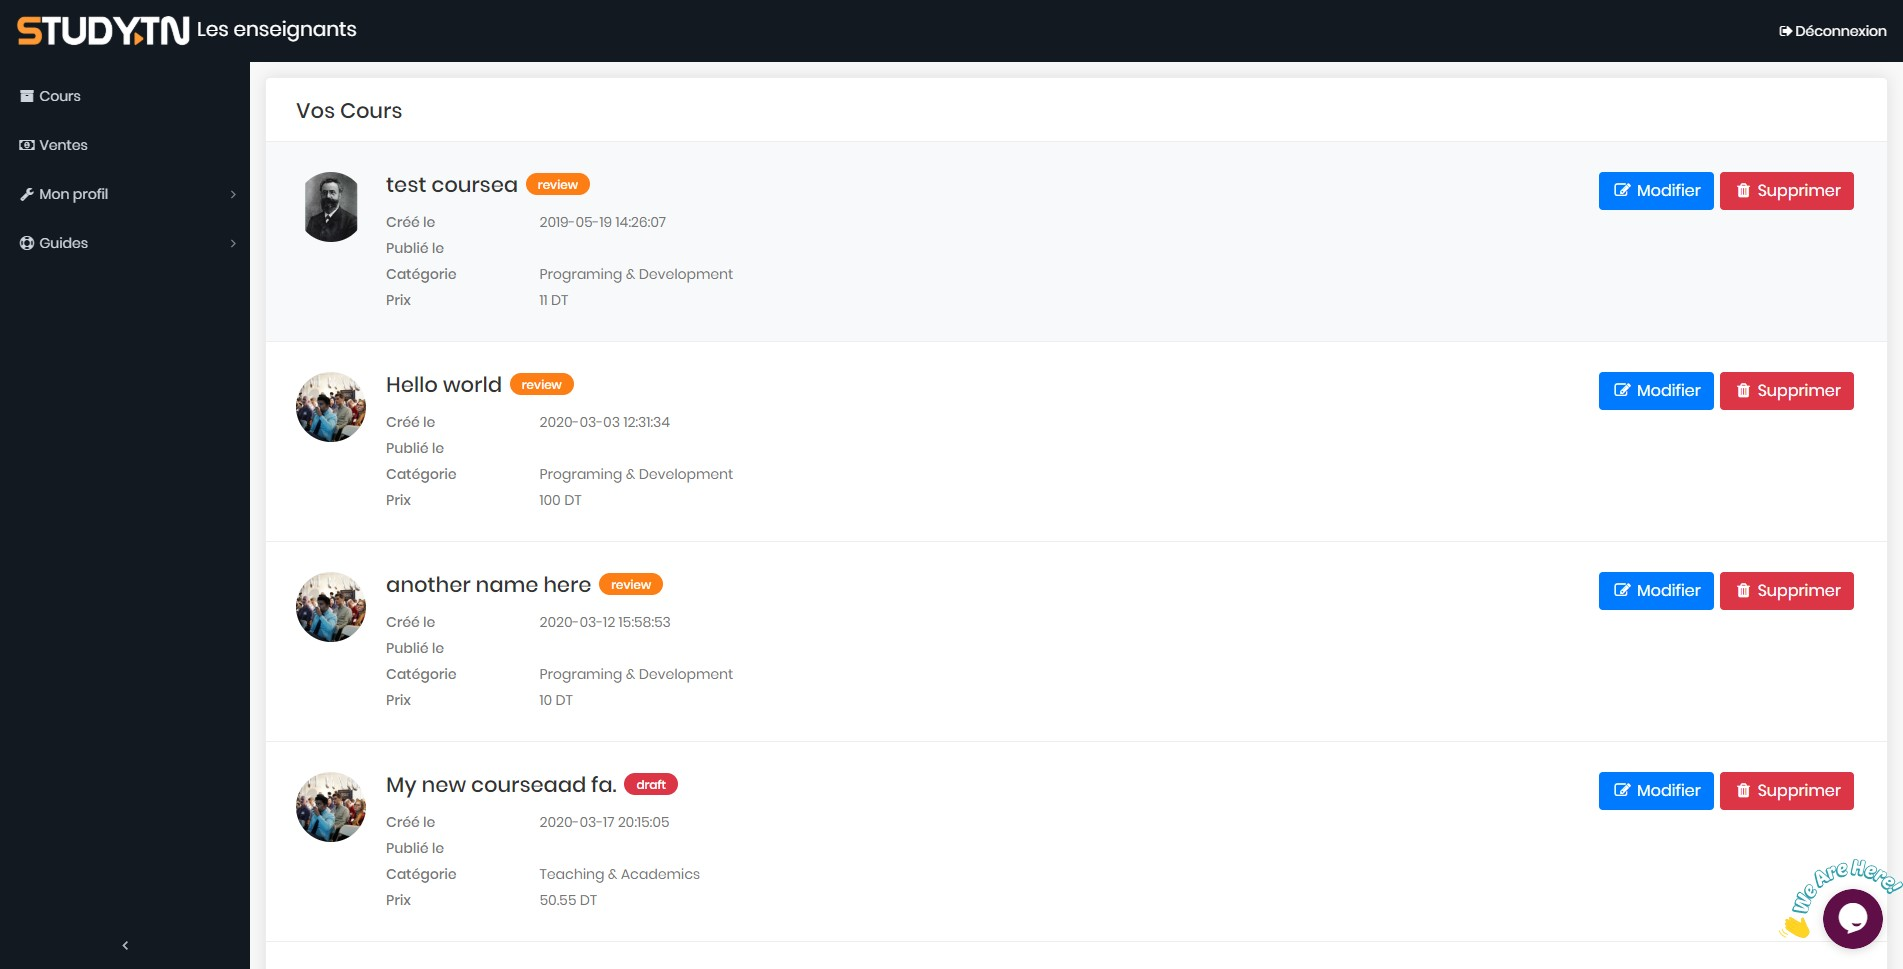
\includegraphics[width=150mm]{currrent_instuctor_space.jpg}
    \caption{The current study.tn instructor dashboard}
    \label{fig:currrent_instuctor_space}
\end{figure}

\subsection{Problem of the existing solutions}
Server-side rendering is a common method for displaying information onto the screen. It works by converting HTML files in the server into usable information for the browser. Whenever you visit a website, your browser makes a request to the server that contains the contents of the website. Once the request is done, your browser will display the rendered HTML on the screen. The current instructor dashboard uses server-side rendering with a template enging which leads to the following issues : 
\begin{itemize}
  \item Touching the front-end risks touching back-end as in theory you can't do a UI rebuilt without messing backend.
  \item Full page reloads when changing routes.
  \item Frequent server requests which The will increase the load on the server.
  \item An overall slow page rendering as the HTML doc gets bigger.

\end{itemize}

\subsection{Proposed solution}
All of the issues above can be overcomed using a front-end framework. We decided to go with react as it is the most used framework for building large scale web applications. Built by Facebook, React makes it simple to create interactive user interfaces. The framework is designed for building component based applications and with the support of backward compatibility, so you can rest assured of its longevity. React has almost 3 million users and a massive developer community. These are the advantages of using react :


\begin{itemize}
  \item Does not require page reloading during use.
  \item Only load the data from the server when needed.
  \item Fast page rendering as it only re-render the components that needs to be updated.
\end{itemize}


%fin code item
\section{Project management}

\subsection{Agile method}
An Agile method is carried out in a collaborative spirit and adapt to incremental approaches. It generates high-quality products while taking into account requirement changes. It also allows
to manage quality continuously and detect problems as soon as possible,
thus allowing corrective actions to be taken without too many penalties in the
costs and deadlines. For our project, we focused on a
Agile type method and more particularly SCRUM\cite{cite0}.

\subsection{Why SCRUM}
SCRUM is a project management method that only presents qualities: 

\begin{itemize}
  \item It is mainly focused on quality, objectives, efficiency.
  \item Minimization of bugs while allowing an excellent communication in the project through the daily Scrum meeting.
  \item The tasks and the "reviewing" process in the project are perfectly defined which totally improves progress.
\end{itemize}


\vfill
\clearpage

\begin{figure}[!ht]
    \centering
    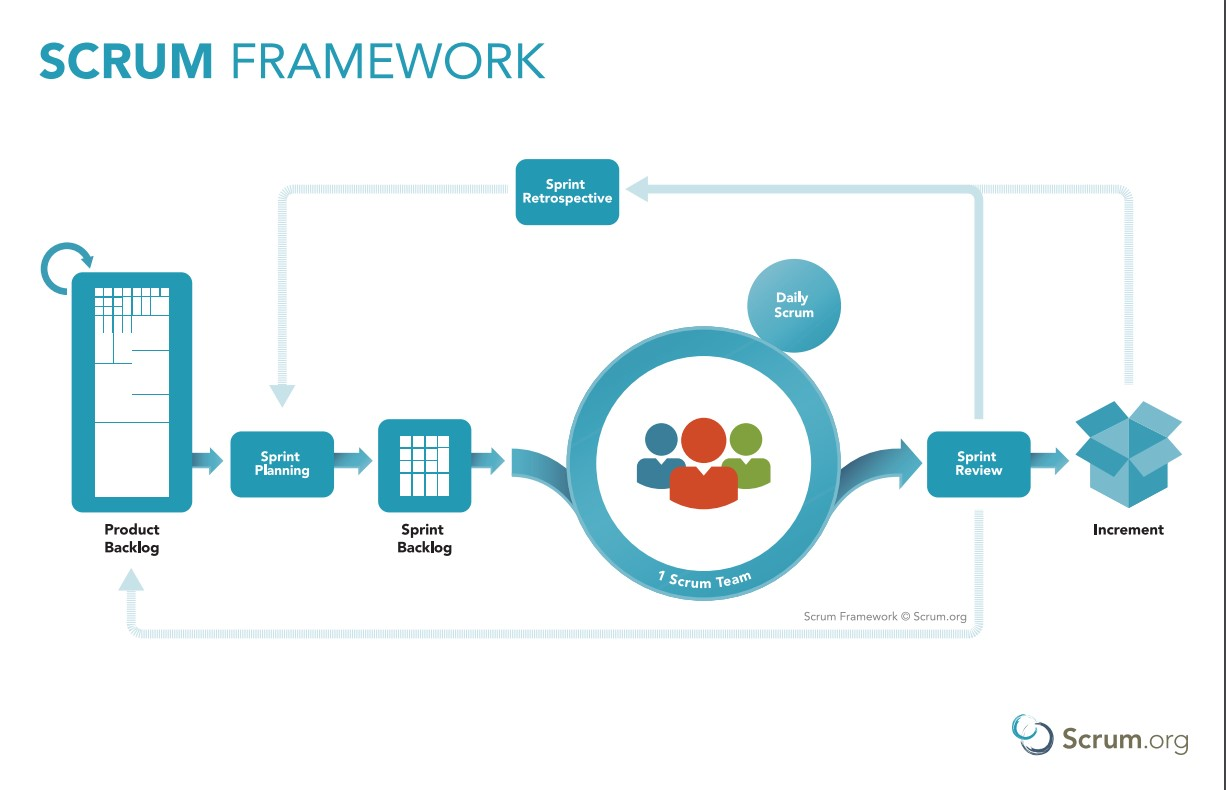
\includegraphics[width=150mm]{scrum.jpg}
    \caption{The Scrum Framework}
    \label{fig:scrum}
\end{figure}



\subsection{UML\cite{cite1}}

UML (Unified Modeling Language) is a formal language normalized in terms of
object modeling.

\subsection{Why UML}
UML brings many advantages such as :
\begin{itemize}
  \item Its independence from programming languages, application and process areas, its versatility and flexibility have made him a universal language.
  \item make the representation and understanding of object solutions easier.
  \item Its graphic notation allows to express an object solution visually, which helps in the comparison and evaluation of solutions.
\end{itemize}

\section*{Conclusion}
Throughout this chapter, we gave a general overview about the project and we have
presented the existing solution and the problems in it. We also introduced the company, the work required and
the chosen methodology. The next chapter will be for the requirements analysis.
        \clearpage
                                
        \chapter{Requirements analysis}
\section*{Introduction}
In this section, we will present the background study of our project in order to identify the
actors who will interact with the system and to list the functional requirements and the non 
functional requirements as well as  our project's backlog and plan our sprints 

\section{Functional requirements}
In the following we will describe the functional requirements of our future system which we will
During this internship, we plan to carry out 
\begin{itemize}
    \item \texbf{Manage system configuration :} The administrator must be able change system configurations (Policies, Visas ..ect)
    \item \texbf{Manage profiles :} The user must be able to change his profile information
    \item \texbf{Create travel orders :} The user must be able to create travel order drafts
    \item \texbf{Manage travel orders :} The agent must be able to change travel orders' status and add attachments 
    \item \texbf{Confirm travel orders :}The manager must be able to confirm travel order drafts and validate the agent's work
\end{itemize}

\section{Non functional requirements}
Apart from the functional requirements that our future system must provide, there is also a
set of non-functional constraints to be respected that represents a desired property of the
system.
Among these requirements are the following: 
\begin{itemize}
\item \textbf{Scalability:} the system must respect a modular architecture where each module
must respond to a set of functionalities covering a common need in order to
to facilitate its reusability for future needs and thus ensure the scalability of the
system
\item \textbf{Security:} our future product must provide a system of restriction on the
manipulations not authorized to a user group with a role defined on the
system
\item \textbf{Internationalization:} our application must have the option of adding more languages
\end{itemize}
\section{Identification of actors}
The system is intended to be used by different users grouped into different profiles:
\begin{itemize}
    \item \textbf{Administrator : }Manages accounts and system configurations
    \item \textbf{User : }Edits his profile and submit travel orders
    \item \textbf{Manager : }Confirm and validate travel orders
    \item \textbf{Agent : }Add reservations to travel orders
\end{itemize}
\section{Project management with Scrum}
   Having opted for Agile SCRUM as our methodology we need to define all actors that take part in the project analysis and implementation and their responsibilities.

\begin{table}[H]
\caption{ Scrum Team }
\begin{tabular}{|p{4,5cm}|p{5,25cm}|p{5,25cm}|}
\hline
\textbf{Role} 
&\textbf{Responsibilities}
&\textbf{Actor}\\
\hline

\hline 
\textbf{- Product Owner} 
&- Identifying core project features\newline{}- Keeping the backlog up-to-date and in priority order\newline{}
&- Amira Hasnaoui\\
\hline

\hline
\textbf{- SCRUM Team} 
&- Modeling\newline{}- Tests and validation\newline{}- Development\newline{}
&- Mohammed Amine ElAmri\\
\hline

\hline
\textbf{- SCRUM Master} 
&- Identify needs and requirments\newline{}- Setup meetings and deadlines
&- Amira Hasnaoui\\
\hline



\end{tabular}
\end{table}
     


	\section{Global project backlog}
	In the following we will present our Product Backlog which will contain the list of
expected system functionality estimate in time and plan according to required priorities
by our Product Owner 
\begin{center}
\begin{longtable}{|p{0.5cm}|p{3.5cm}|p{6,5cm}|p{2cm}|p{2cm}|}
\caption{ Project backlog }
\hline
\textbf{ID} 
&\textbf{Theme}
&\textbf{User Story}
&\textbf{Estimation}
&\textbf{Priority}\\
\hline
1
&Authentification
&As an Administrator , Agent , Manager or User, I want to be able to log-in
&12h
&HIGH
\hline

2
&\multirow{4}{*}{\begin{tabular}[c]{@{}l@{}}Account Managment\end{tabular}}
&As an Administrator, I want to be able to create user accounts
&8h
&HIGH\\ \cline{1-1} \cline{3-5} 

3
&
&As an Administrator, I want to be able to edit user details
&4h
&LOW\\
\cline{1-1} \cline{3-5} 
4
&
&As a Manager, I want to be able to edit user roles
&4h
&LOW\\
\cline{1-1} \cline{3-5} 
5
&
&As an Administrator, I want to be able to view the users list
&10h
&MEDIUM\\
\hline
6
&\multirow{2}{*}{\begin{tabular}[c]{@{}l@{}}Profile Managment\end{tabular}}
&As a User , I want to be able to view my profile details
&8h
&HIGH\\
\cline{1-1} \cline{3-5} 
7
&
&As a User , I want to be able to change my profile details
&2h
&LOW\\
\hline
8
&\multirow{11}{*}{\begin{tabular}[c]{@{}l@{}}Configuration\end{tabular}}
&As an Administrator , I want to be able to view, create, edit, delete and import new countries
&16h
&HIGH\\
\cline{1-1} \cline{3-5} 
9
&
&As an Administrator , I want to be able to view, create, edit, delete and import flight policies
&8h
&MEDIUM\\
\cline{1-1} \cline{3-5} 
10
&
&As an Administrator , I want to be able to view, create, edit, delete and import hotel reservation policy
&8h
&MEDIUM\\
\cline{1-1} \cline{3-5} 
11
&
&As an Administrator , I want to be able to view, create, edit, delete and import per diem policy
&8h
&MEDIUM\\
\cline{1-1} \cline{3-5} 
12
&
&As an Administrator , I want to be able to view, create, edit, delete and import visa models
&6h
&LOW\\
\cline{1-1} \cline{3-5} 
13
&
&As an Administrator , I want to be able to view, create, edit, delete and import vaccins
&6h
&LOW\\
\cline{1-1} \cline{3-5} 
14
&
&As an Administrator , I want to be able to attribute vaccines to countries
&6h
&LOW\\
\cline{1-1} \cline{3-5} 
15
&
&As an Administrator , I want to be able to attribute visas to countries
&6h
&LOW\\
\cline{1-1} \cline{3-5} 
16
&
&As an Administrator , I want to be able to create , edit and delete administrative grades
&8h
&MEDIUM\\
\cline{1-1} \cline{3-5} 
17
&
&As an Administrator , I want to be to attribute administrative grades to users
&6h
&LOW\\
\cline{1-1} \cline{3-5} 
18
&
&As an Administrator , I want to be able to create , edit and delete mission types
&8h
&LOW\\
\hline
19
&\multirow{10}{*}{\begin{tabular}[c]{@{}l@{}}Travel Order \\Managment\end{tabular}}
&As a User , I want to be able to create , edit and delete travel order drafts
&16h
&HIGH\\
\cline{1-1} \cline{3-5} 
20
&
&As a User , I want to be able to see all my travel orders
&10h
&MEDIUM\\
\cline{1-1} \cline{3-5} 
21
&
&As a User , I want to be able to filter my travel orders by status or date
&6h
&LOW\\
\cline{1-1} \cline{3-5} 
22
&
&As a User , I want to be able to file my travel order drafts and track their progress
&10h
&HIGH\\
\cline{1-1} \cline{3-5} 
23
&
&As an Agent , I want to be able to see all travel orders,
&8h
&MEDIUM\\
\cline{1-1} \cline{3-5} 
24
&
&As an Agent , I want to be able to add attachments to travel orders
&12h
&MEDIUM\\
\cline{1-1} \cline{3-5} 
25
&
&As an Agent , I want to be able to change travel orders' status
&10h
&MEDIUM\\
\cline{1-1} \cline{3-5} 
26
&
&As a Manager , I want to be able to see all travel orders pending my confirmation
&10h
&MEDIUM\\
\cline{1-1} \cline{3-5} 
27
&
&As a Manager , I want to be able to confirm or reject travel orders pending my confirmation
&12h
&MEDIUM\\
\hline
\end{longtable}

\end{center}
    \section{Sprints planning}
    \\Our project lasts three months and follows the Scrum methodology that we have chosen as our working methodology, We can estimate our project on four main phases which are:
    \begin{itemize}
        \item \textbf{Sprint 0 :} Preliminary Phase
        \begin{itemize}
\item Identification of actors
\item Global analysis
\item development environment choices and configuration of the work environment
\item The architectural model
\item Product Backlog
        \end{itemize}
        \item \textbf{Sprint 1 :} Configuration Module
        \begin{itemize}
\item Sprint Backlog 
\item detailed design of the target module
\item Implementation
        \end{itemize}
        \item \textbf{Sprint 2 :} Employee Module
        \begin{itemize}
\item Sprint Backlog 
\item detailed design of the target module
\item Implementation
        \end{itemize}
        \item \textbf{Sprint 3 :} Travel order Module
        \begin{itemize}
\item Sprint Backlog 
\item detailed design of the target module
\item Implementation
        \end{itemize}
    \end{itemize}
    
    \begin{table}[H]
    \begin{tabular}{|p{4cm}|p{6,5cm}|p{4cm}|}
    \hline
\textbf{Sprint} 
&\textbf{User Stories}
&\textbf{Estimation}\\
\hline
Sprint 1
&US1 , US8 , US9 ,  US10 , US11 , US12 , US13 , US14 , US15 , US16 , US17 , US18
&4 weeks\\
\hline
Sprint 2
&US2 , US3 , US4 , US5 , US6 , US7
&3 weeks\\
\hline
Sprint 3
&US19 , US20 , US21 ,  US22 , US23 , US24 , US25 , US26 , US27 
&5 weeks\\
\hline
\end{tabular}
\end{table}


    \section{Project Structure}
    \subsection*{Actors}
    The diagram below helps to highlight the relationships between the different actors
     \begin{figure}[H]
    \begin{center}
        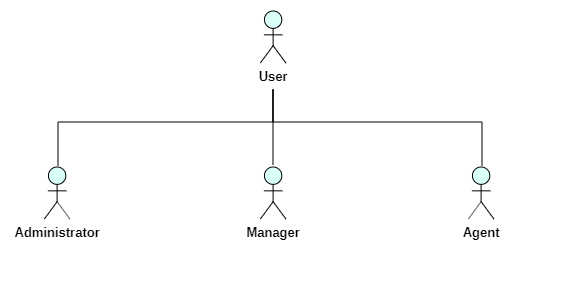
\includegraphics[scale=0.6]{img/actors.png}
        \caption{Actors relationship diagram}
    \end{center}
    \end{figure}
    \subsection*{Global usecase diagram}
    The use case diagram below helps to highlight the relationships between the actors and the system under study
    \begin{figure}[H]
    \begin{center}
        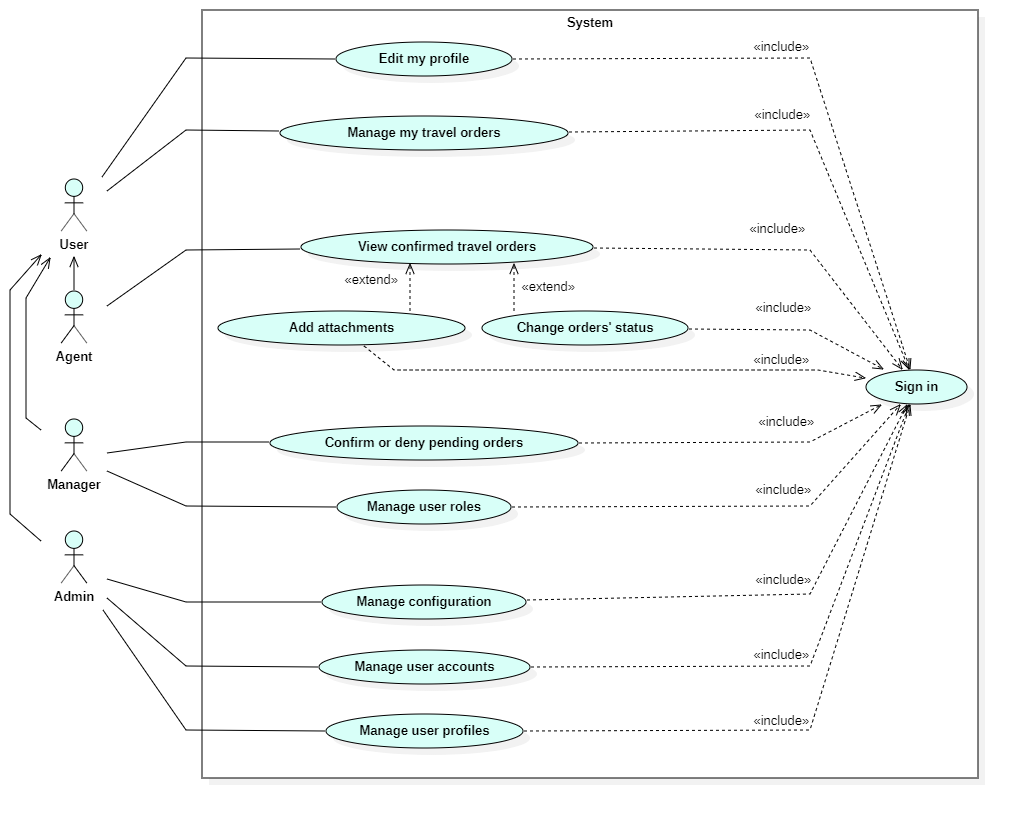
\includegraphics[scale=0.48]{img/global_usecase.png}
        \caption{global use case diagram}
    \end{center}
    \end{figure}
    
\section*{Conclusion}
This chapter summarizes the preliminary study we conducted before entering the development phase of our system. First we identified the actors who interact with the application, then we identified the functional needs and the non-functional requirements. Then we presented our product backlog and the breakdown of our project.\\
We concluded the chapter with UML diagrams to formulate these requirements.

    
        \clearpage
        
        \chapter{Sprint Zero - HARDWARE AND SOFTWARE ENVIRONMENT}
\newpage
\section*{Introduction}
This chapter will cover the hardware and software environment the project was built on.
\addcontentsline{toc}{section}{Introduction}
\section{Hardware environment}
The project was built on a desktop computer with the following specs :

\begin{itemize}
  \item Processor : Intel i7-7700 Processor (8M Cache, up to 4.20 GHz)
  \item RAM : 8 GB DDR4 3200 MHZ
  \item Graphic card : GTX  1070 8gb GDDR5
  \item Operating system : Windows 10 64 bits
\end{itemize}
\section{Software environment}

\hfill \break
\textbf{React \cite{cite3} :} React is a JavaScript library for building user interfaces. React allows developers to create large web applications that can change data, without reloading the page. The main purpose of React is to be fast, scalable, and simple. It works only on user interfaces in the application. This corresponds to the view in the MVC template.


\textbf{Redux \cite{cite4} :} Redux itself is a standalone library that can be used with any UI layer or framework, including React, Angular, Vue, Ember, and vanilla JS. Although Redux and React are commonly used together, they are independent of each other. It's predictable state container for JavaScript apps.

\hfill \break
\hfill \break
\textbf{Node \cite{cite2} :} Node.js is an open-source, cross-platform, JavaScript runtime environment that executes JavaScript code outside a web browser. Node is required to work with react.

\hfill \break
\hfill \break
\textbf{Adobe XD \cite{cite9} :} XD empowers designers with the speed, precision, and quality to seamlessly iterate and share interactive prototypes with team members and reviewers across devices and platforms, including Windows, Mac, iOS, and Android. We will use that to open and work with the wireframes shown previously.

\vfill
\clearpage

\begin{figure}[!ht]
    \centering
    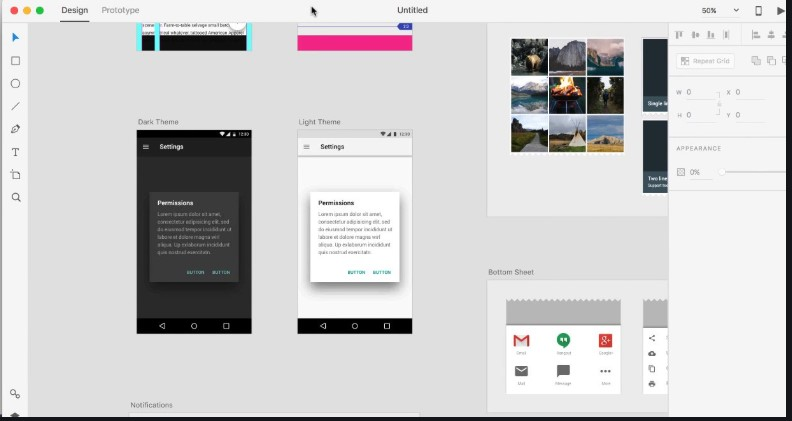
\includegraphics[width=150mm]{adobexd_interface.jpg}
    \caption{Adobe XD interface}
    \label{fig:adobexd_interface}
\end{figure}

\hfill \break
\hfill \break
\textbf{Visual Studio Code \cite{cite7} :} is an opensource text/code editor developed by Microsoft for Windows, Linux and MacOs. It is one of the best code editors in the market given its speed, the variation of the proposed extensions and the integrated terminal. It also supports several languages and Frameworks such as NodeJS and React.

\begin{figure}[!ht]
    \centering
    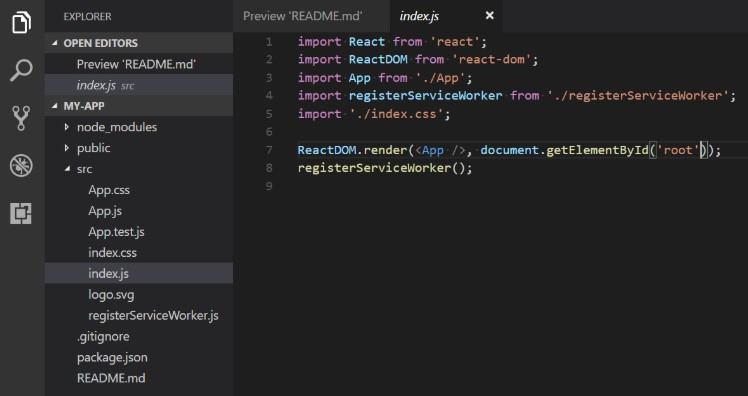
\includegraphics[width=170mm]{visual_code_interface.jpg}
    \caption{Visual Studio interface}
    \label{fig:visual_code_interface}
\end{figure}

\hfill \break
\hfill \break
\textbf{Postman \cite{cite5} :} Postman is a software development tool. It enables people to test calls to APIs. Postman users enter data. The data is sent to a special web server address. Typically, information is returned, which Postman presents to the user.

\begin{figure}[!ht]
    \centering
    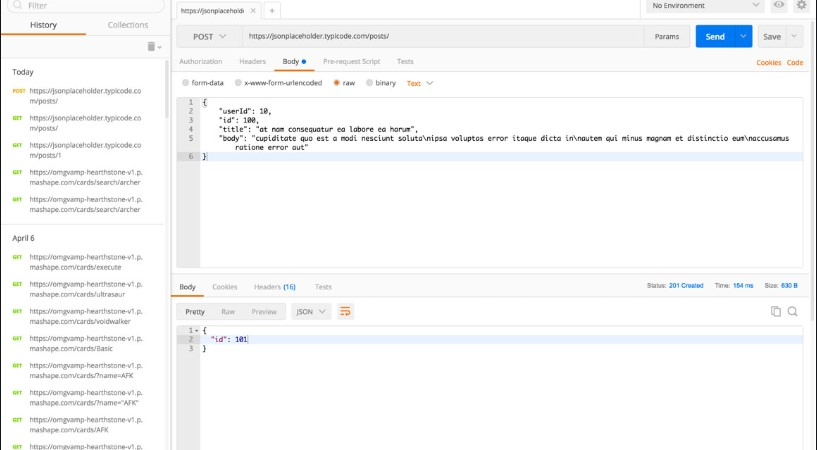
\includegraphics[width=150mm]{postman_interface.jpg}
    \caption{Postman interface}
    \label{fig:postman_interface}
\end{figure}


\hfill \break
\hfill \break
\textbf{Gitlab \cite{cite8} :} is a Git repository hosting service, but it adds many of its own features. While Git is a command line tool, Gitlab provides a Web-based graphical interface. It also provides access control and several collaboration features, such as a wikis and basic task management tools for every project.


\begin{figure}[!ht]
    \centering
    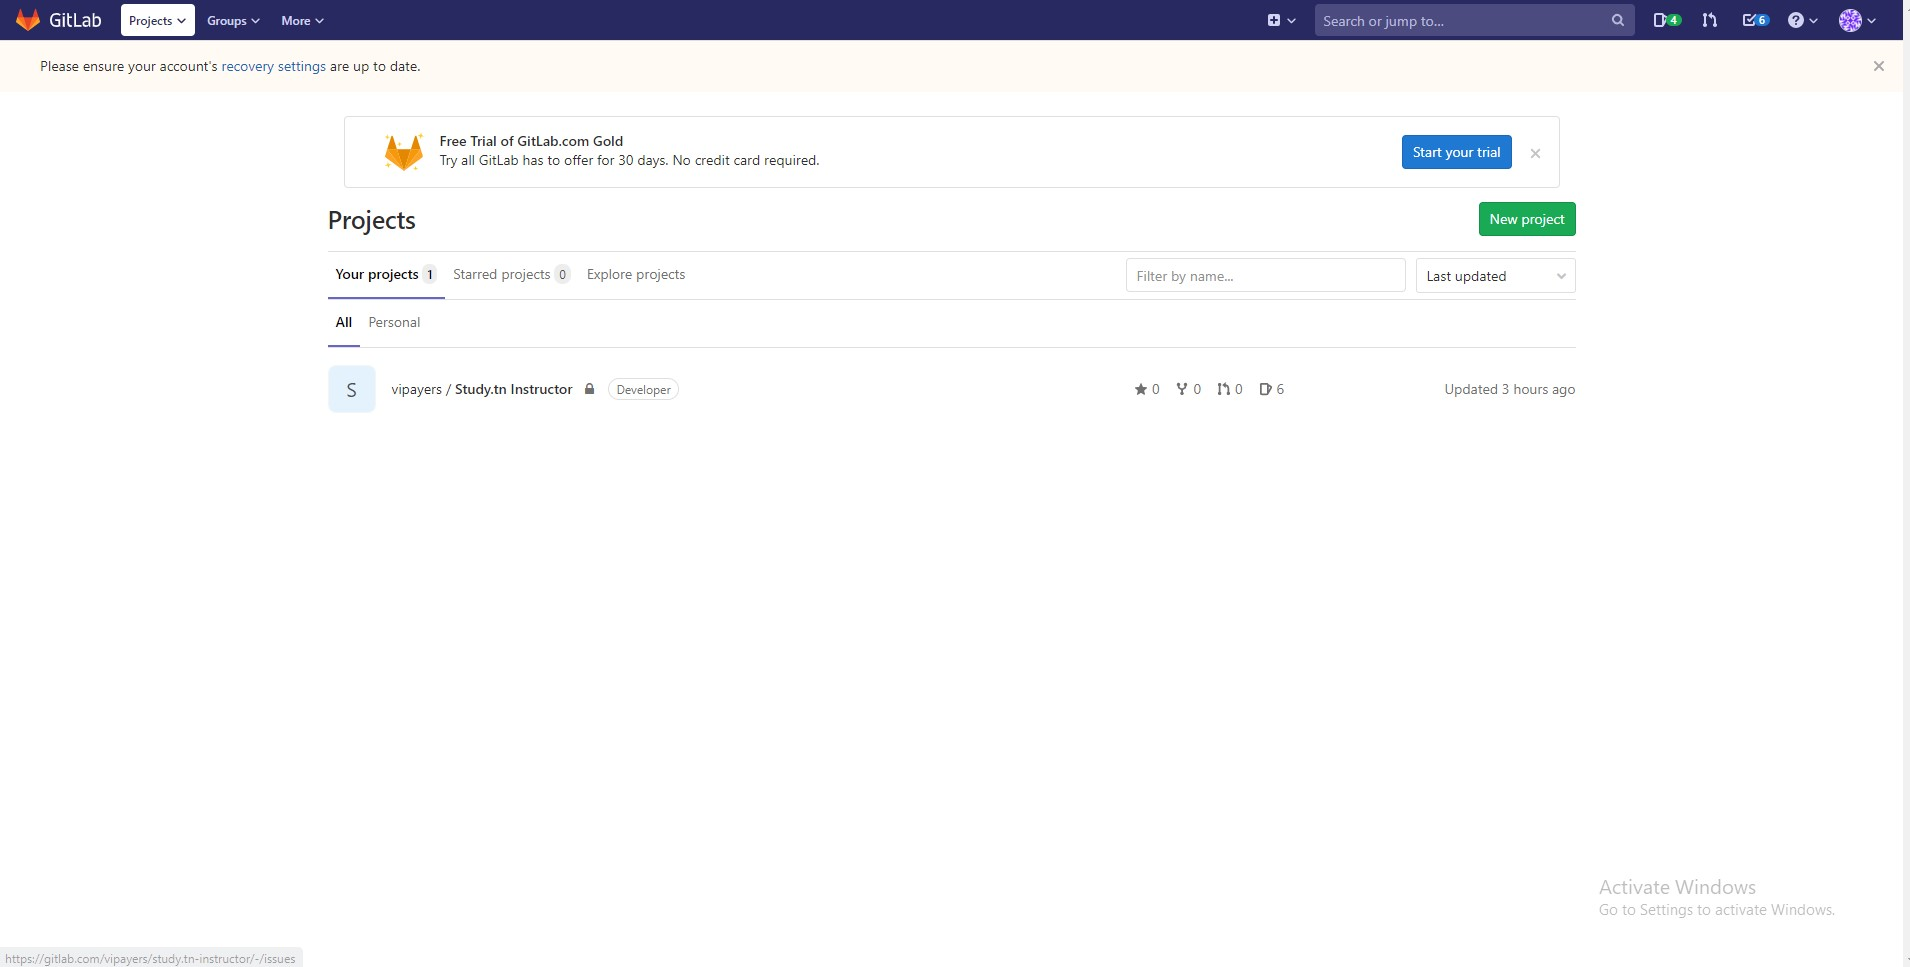
\includegraphics[width=150mm]{gitlab_interface.jpg}
    \caption{Gitlab interface}
    \label{fig:gitlab_interface}
\end{figure}

\vfill
\clearpage

\hfill \break
\hfill \break
\textbf{Slack \cite{cite6} :} Slack is a collaboration hub that can replace email to help you and your team work together seamlessly. It’s designed to support the way people naturally work together, so you can collaborate with people online as efficiently as you do face-to-face.

\begin{figure}[!ht]
    \centering
    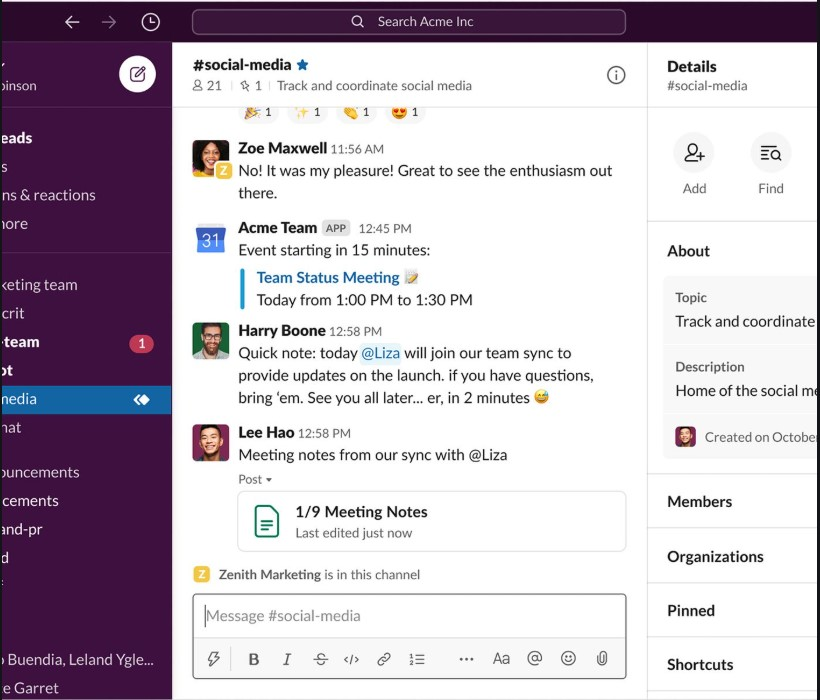
\includegraphics[width=150mm]{slack_interface.jpg}
    \caption{Slack interface}
    \label{fig:slack_interface}
\end{figure}


\section{Application architecture}

\vfill
\clearpage

\begin{figure}[!ht]
    \centering
    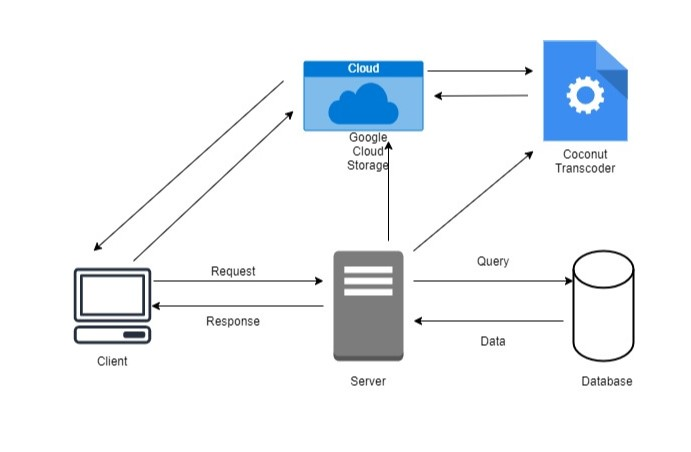
\includegraphics[width=150mm]{project_architecture.jpg}
    \caption{Application architecture}
    \label{fig:slack_interface}
\end{figure}



\section*{Conclusion}
In this chapter, we have presented our hardware and software environment, and the different tools used to build our project. In the next chapter, we will cover the first sprint which will be about the course management.

        \clearpage
        
        \chapter{Sprint 1}

\section*{Introduction}
In this Sprint we go through the planning, analyzing, and implementing phases of the configuration module.
\subsubsection*{Purpose of the configuration module}
This module is dedicated to the platform administrator. \\
It is a parameter setting module that facilitates the internal configuration of the application, mainly by managing :\\
\begin{itemize}
    \item The different travel policies
    \item The destinations and their requirements (visa and vaccines)
    \item The administrative grades
\end{itemize}\\
\subsubsection*{Actors}
There is a single actor that can access and interact with this module:
\begin{itemize}
    \item Admin: The platform's administrator
\end{itemize}\\
\section{Sprint backlog}
The following table summarizes the tasks that we are responsible for carrying out 
\begin{center}
\begin{longtable}{|p{1cm}|p{6,25cm}|p{0,7cm}|p{6,25cm}|p{0,8cm}|}
\caption{ Project backlog }
\hline
\textbf{US ID} 
&\textbf{User Story}
&\textbf{T ID}
&\textbf{Task}
&\textbf{Esti- ma- tion}
\\
\hline
\multirow{ 3}{*}{0}
&\multirow{3}{*}{Storyless}
&0.1
&Class diagram
&8h\\\cline{3-5}
&
&0.2
&Use case diagram
&8h\\\cline{3-5}
&
&0.3
&Documenting progress
&2h\\\cline{3-5}
\hline
1
&As an Administrator , Agent , Manager or User, I want to be able to log-in
&1
&Setup Odoo
&8h
\\\hline


\multirow{ 6}{*}{8}
&\multirow{6}{=}{As an Administrator , I want to be able to view, create, edit, delete and import new countries}
&8.1
&Create the «country» model
&8h\\\cline{3-5}
&
&8.2
&Create the view
&2h\\\cline{3-5}
&
&8.3
&Create security rules
&1h\\\cline{3-5}
&
&8.4
&Create the «Destinations» menu item
&30m\\\cline{3-5}
&
&8.5
&Create the «Airport» model
&30m\\\cline{3-5}
&
&8.6
&Create the «State» model
&30m\\\cline{3-5}
\hline


\multirow{ 5}{*}{9}
&\multirow{5}{=}{As an Administrator , I want to be able to view, create, edit, delete and import flight policies}
&9.1
&Create the «flight\_policy» model
&8h\\\cline{3-5}
&
&9.2
&Create the view
&2h\\\cline{3-5}
&
&9.3
&Create security rules
&1h\\\cline{3-5}
&
&9.4
&Create the «Policies» menu item
&30m\\\cline{3-5}
&
&9.5
&Create «flight\_class\_rules» model
&4h\\\cline{3-5}
\hline


\multirow{ 3}{*}{10}
&\multirow{3}{=}{As an Administrator , I want to be able to view, create, edit, delete and import hotel reservation policy}
&10.1
&Create the «hotel\_policy» model
&8h\\\cline{3-5}
&
&10.2
&Create the view
&2h\\\cline{3-5}
&
&10.3
&Create security rules
&1h\\\cline{3-5}

\hline
\multirow{3}{*}{11}
&\multirow{3}{=}{As an Administrator , I want to be able to view, create, edit, delete and import per diem policy}
&11.1
&Create the «perdiem\_policy» model
&8h\\\cline{3-5}
&
&11.2
&Create the view
&2h\\\cline{3-5}
&
&11.3
&Create security rules
&1h\\\cline{3-5}
\hline

\multirow{ 4}{*}{12}
&\multirow{4}{=}{As an Administrator , I want to be able to view, create, edit, delete and import visa model}
&12.1
&Create the «visa» model
&8h\\\cline{3-5}
&
&12.2
&Create the view
&2h\\\cline{3-5}
&
&12.3
&Create security rules
&1h\\\cline{3-5}
&
&12.4
&Create model relations
&2h\\\cline{3-5}
\hline


\multirow{ 4}{*}{13}
&\multirow{4}{=}{As an Administrator , I want to be able to view, create, edit, delete and import vaccins}
&13.1
&Create the «vaccine» model
&4h\\\cline{3-5}
&
&13.2
&Create the view
&1h\\\cline{3-5}
&
&13.3
&Create security rules
&1h\\\cline{3-5}
&
&13.4
&Create the «Vaccine» menu item
&30m\\\cline{3-5}

\hline

14
&As an Administrator , I want to be able to attribute vaccines to countries
&14.1
&Create model relation
&2h\\
\hline

15
&As an Administrator , I want to be able to attribute visas to countries
&15.1
&Create model relation
&2h\\
\hline
\\\\

\multirow{5}{*}{16}
&\multirow{5}{=}{As  an  Administrator  ,  I  want  to be able to create , edit and delete administrative grades}
&16.1
&Create the «grade» model
&8h\\\cline{3-5}
&
&16.2
&Create the view
&30m\\\cline{3-5}
&
&16.3
&Create security rules
&1h\\\cline{3-5}
&
&16.4
&Create model relations
&1h\\\cline{3-5}
&
&16.5
&Create the «Grade» menu item
&30m\\\cline{3-5}
\hline

\multirow{ 3}{*}{17}
&\multirow{3}{=}{As an Administrator , I want to be to attribute administrative grades to users}
&17.1
&Add «Grade» field to «hr\_employee» model
&4h\\\cline{3-5}
&
&17.2
&edit «hr\_employee» security rules
&2h\\\cline{3-5}
&
&17.3
&edit «hr\_employee» view
&1h\\\cline{3-5}
\hline

\multirow{ 3}{*}{18}
&\multirow{3}{=}{As an Administrator , I want to be able to create , edit and delete mission types}
&18.1
&Create the «mission\_type» model
&8h\\\cline{3-5}
&
&18.2
&Create the view
&2h\\\cline{3-5}
&
&18.3
&Create security rules
&1h\\\cline{3-5}
\hline
\end{longtable}
\end{center}
\section{Software Design}
The conceptual study conducted at the beginning of an iteration allows us to evaluate the sprint in its early stages by providing a stable reference of conceptual data model and processing to identify potential scenarios. 
    \subsection{Class diagram}
    The following diagram represents the entities manipulated by users as
analysis class diagram
    \begin{figure}[H]
    \begin{center}
        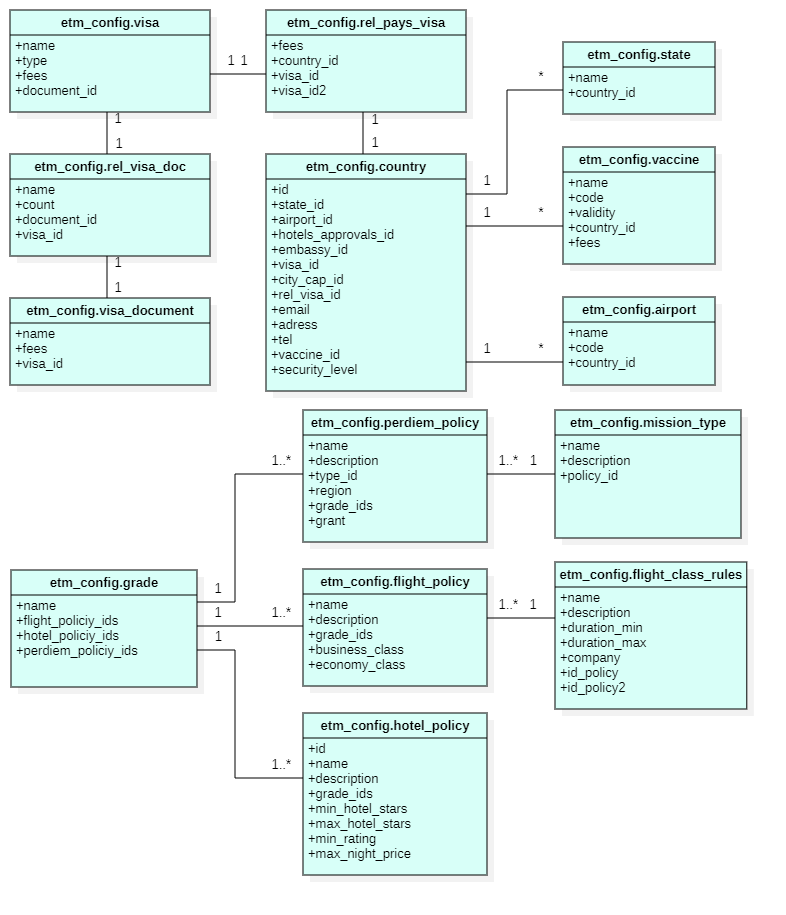
\includegraphics[scale=0.5]{img/sprint1_class.png}
        \caption{Sprint 1 class diagram}
    \end{center}
     \label{fig:my_label}
\end{figure}
    \subsection{Use case diagram}
    The use case diagram below helps to highlight the relationships
functional between the actors and the system under study 
    \begin{figure}[H]
    \begin{center}
        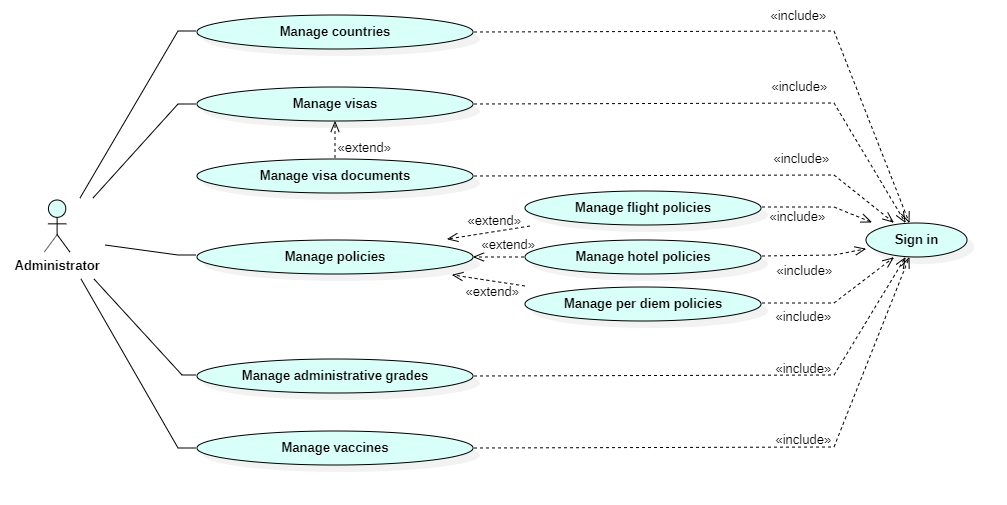
\includegraphics[scale=0.50]{img/UseCaseDiagramSprint1.png}
        \caption{Sprint 1 use case diagram}
    \end{center}
        \label{fig:my_label}
\end{figure}
  \\ In what follows, we will proceed to go in detail on some use cases  


\subsection*{Use case «Manage countries»}
\begin{figure}[H]
    \begin{center}
        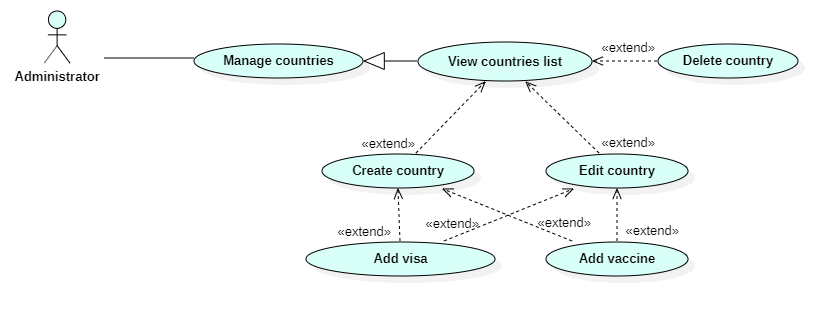
\includegraphics[scale=0.5]{img/sprint1_country_usecase.png}
        \caption{«Manage countries» detailed use case diagram}
    \end{center}
        \label{fig:my_label}
\end{figure} 
    The following table addresses the use case previously illustrated by providing a textual description, post and preconditions as well as the main scenario and the nominal scenario
    \begin{center}
    
\begin{longtable}{|p{4,25cm}|p{9,25cm}|}
\caption{«Manage countries» detailed textual description}
\hline
\textbf{Use Case}&Create country
\\\hline
\textbf{Actors}&Administrator
\hline
\textbf{Pre-condition}&Administrator signed in and viewing countries list
\hline
\textbf{Post-condition}&New country created
\hline
\textbf{Basic path}&
        \begin{itemize}
         \item[1.] The administrator clicks on the button "New"
         \item[2.] The system displays a form to fill out
         \item[3.] The administrator fills the form
         \item[4.] The administrator clicks on the button "Save"
         \item[5.] The system processes the input
         \item[6.] The system saves the new country
         \item[7.] The administrator is sent back to the countries list
     \end{itemize}\\
\hline
\textbf{Alternative path}&
\begin{itemize}
\item 4.Duplicate or missing Data (The administrator is sent back to step 2)

\end{itemize}\\
\hline
\end{longtable}
\end{center}




\subsection*{Use case «Manage visas»}
\begin{figure}[H]
    \begin{center}
        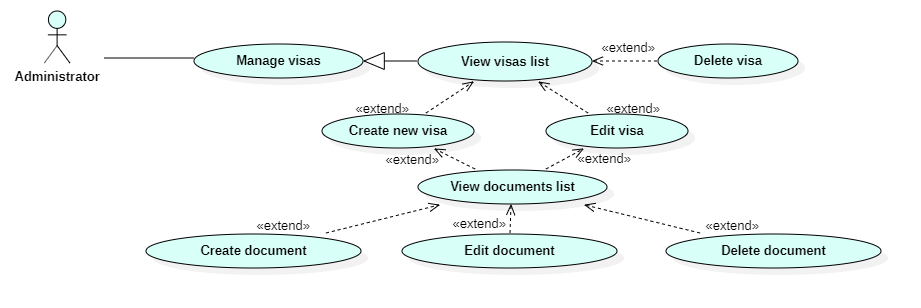
\includegraphics[scale=0.45]{img/sprint1_visa_usecase.png}
        \caption{«Manage visas» detailed use case diagram}
    \end{center}    
\end{figure}
    In the following we will present the sequence diagram to illustrate the relationships between the actor and the different components of our use case from a temporal point of view, focusing on the chronology of the exchanges of messages.
    \begin{figure}[H]
     \begin{center}
        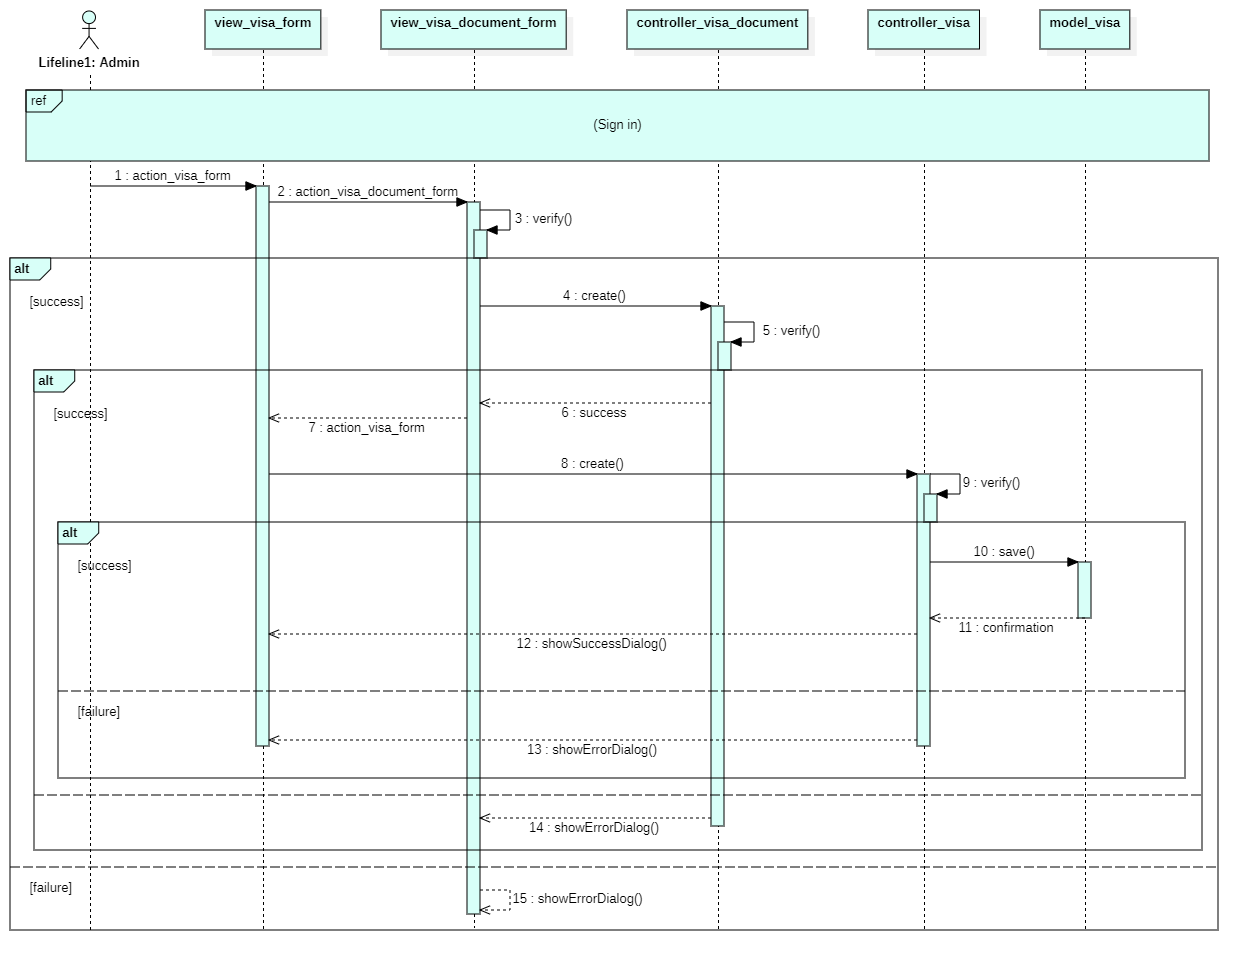
\includegraphics[scale=0.355]{img/sprint1_visa_sequ.png}
        \caption{«Manage visas» sequence diagram}
    \end{center}   
    \end{figure}
    
    
    
    
    
\subsection*{Use case «Manage vaccines»}
\begin{figure}[H]
    \begin{center}
        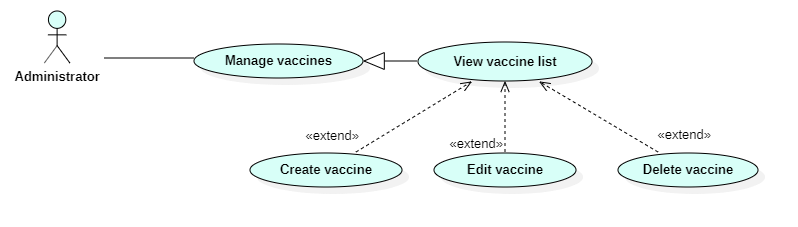
\includegraphics[scale=0.50]{img/sprint1_vaccine_usecase.png}
 \caption{«Manage vaccines» detailed use case diagram}
    \end{center}   
    \end{figure}
      The following table addresses the use case previously illustrated by providing a textual description, post and preconditions as well as the main scenario and the nominal scenario
    \begin{center}
    
\begin{longtable}{|p{4,25cm}|p{9,25cm}|}
\caption{«Manage vaccines» detailed textual description}
\hline
\textbf{Use Case}&Create vaccine
\\\hline
\textbf{Actors}&Administrator
\hline
\textbf{Pre-condition}&Administrator signed in and viewing vaccines list
\hline
\textbf{Post-condition}&New vaccine created
\hline
\textbf{Basic path}&
        \begin{enumerate}
         \item The administrator clicks on the button "New"
         \item The system displays a form to fill out
         \item The administrator fills the form
         \item The administrator clicks on the button "Save"
         \item The system processes the input
         \item The system saves the new vaccine
         \item The administrator is sent back to the countries list
     \end{enumerate}\\
\hline
\textbf{Alternative path}&
\begin{itemize}
\item 4.Duplicate or missing Data (The administrator is sent back to step 2)

\end{itemize}\\
\hline
\end{longtable}
\end{center}  
    
    
    
    
    
    
    
\subsection*{Use case «Manage policies»}
\begin{figure}[H]
    \begin{center}
        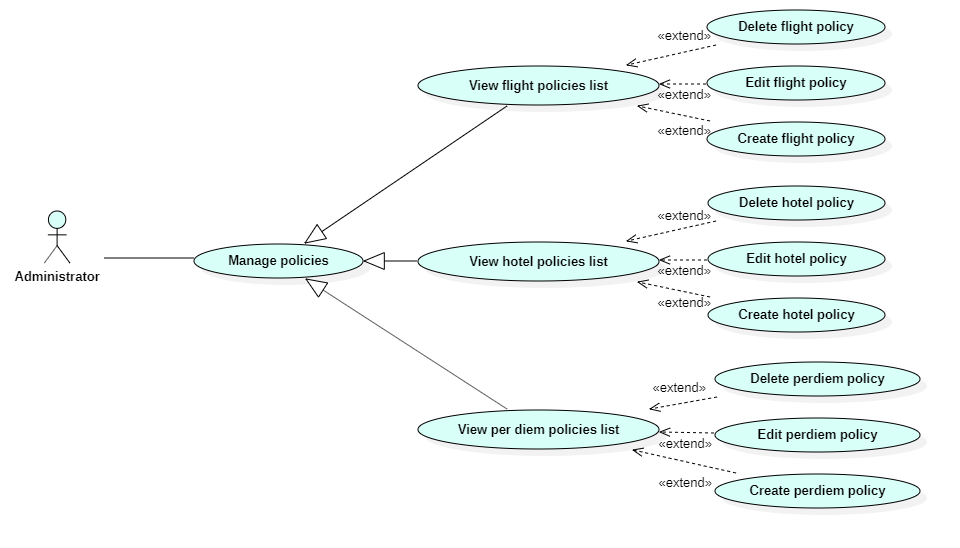
\includegraphics[scale=0.50]{img/sprint1_policy_usecase.png}
         \caption{«Manage policies» detailed use case diagram}
    \end{center}   
    \end{figure}
    
    
        \begin{center}
    
\begin{longtable}{|p{3.2cm}|p{10cm}|}
\caption{«Manage policies» detailed textual description}
\hline
\textbf{Use Case}&Edit flight policy
\\\hline
\textbf{Actors}&Administrator
\hline
\textbf{Pre-condition}&Administrator signed in and flight policies list
\hline
\textbf{Post-condition}&Flight policy edited\\
\hline
\textbf{Basic path}&
        \begin{enumerate}
         \item The administrator clicks on the button "New"
         \item The system displays a form to fill out
         \item The administrator fills the form
         \item The administrator selects at least one of each policy
         \item The administrator clicks on the button "Save"
         \item The system processes the input
         \item The system saves the new vaccine
         \item The administrator is sent back to the countries list
     \end{enumerate}\\
\hline
\textbf{Alternative path}&
\begin{itemize}
\item 6.Duplicate or missing Data (The administrator is sent back to step 3)
\item 4.No policy exist and the user is prompted to go to the policy creation form
\end{itemize}\\
\hline
\end{longtable}
\end{center}  




\subsection*{Use case «Manage administrative grades»}
\begin{figure}[H]
    \begin{center}
        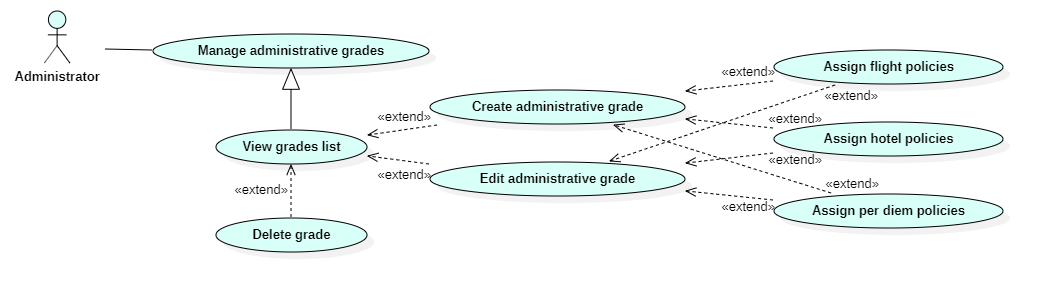
\includegraphics[scale=0.50]{img/sprint1_grade_usecase.png}
        \caption{«Manage administrative grades» detailed use case diagram}
    \end{center}   
    \end{figure}
    
    The following table addresses the use case previously illustrated by providing a textual description,post and preconditions as well as the main scenario and the nominal scenario
    
            \begin{center}
    
\begin{longtable}{|p{3.2cm}|p{10cm}|}
\caption{«Manage administrative grades» detailed textual description}
\hline
\textbf{Use Case}&Create administrative grade
\\\hline
\textbf{Actors}&Administrator
\hline
\textbf{Pre-condition}&Administrator signed in and viewing grades list
\hline
\textbf{Post-condition}&New grade created
\hline
\textbf{Basic path}&
        \begin{enumerate}
         \item The administrator selects a policy
         \item The system displays the policy information
         \item The administrator clicks on the button "Edit"
         \item The system displays a filled form
         \item The administrator edits the fields
         \item The administrator clicks on the button "Save"
         \item The system processes the input
         \item The system saves the new policy
         \item The administrator is sent back to the flight policies list
     \end{enumerate}\\
\hline
\textbf{Alternative path}&
\begin{itemize}
\item 7.Duplicate or missing Data (The administrator is sent back to step 3)
\item 6.form not edited (System skips to step 9)
\end{itemize}\\
\hline
\end{longtable}
\end{center}  



\section{Implementation}
This section presents some user interfaces of the module with screenshots to further clarify our work. The figures below present these interfaces, starting with the first figure which shows the authentication interface.

\begin{figure}[H]
    \centering
    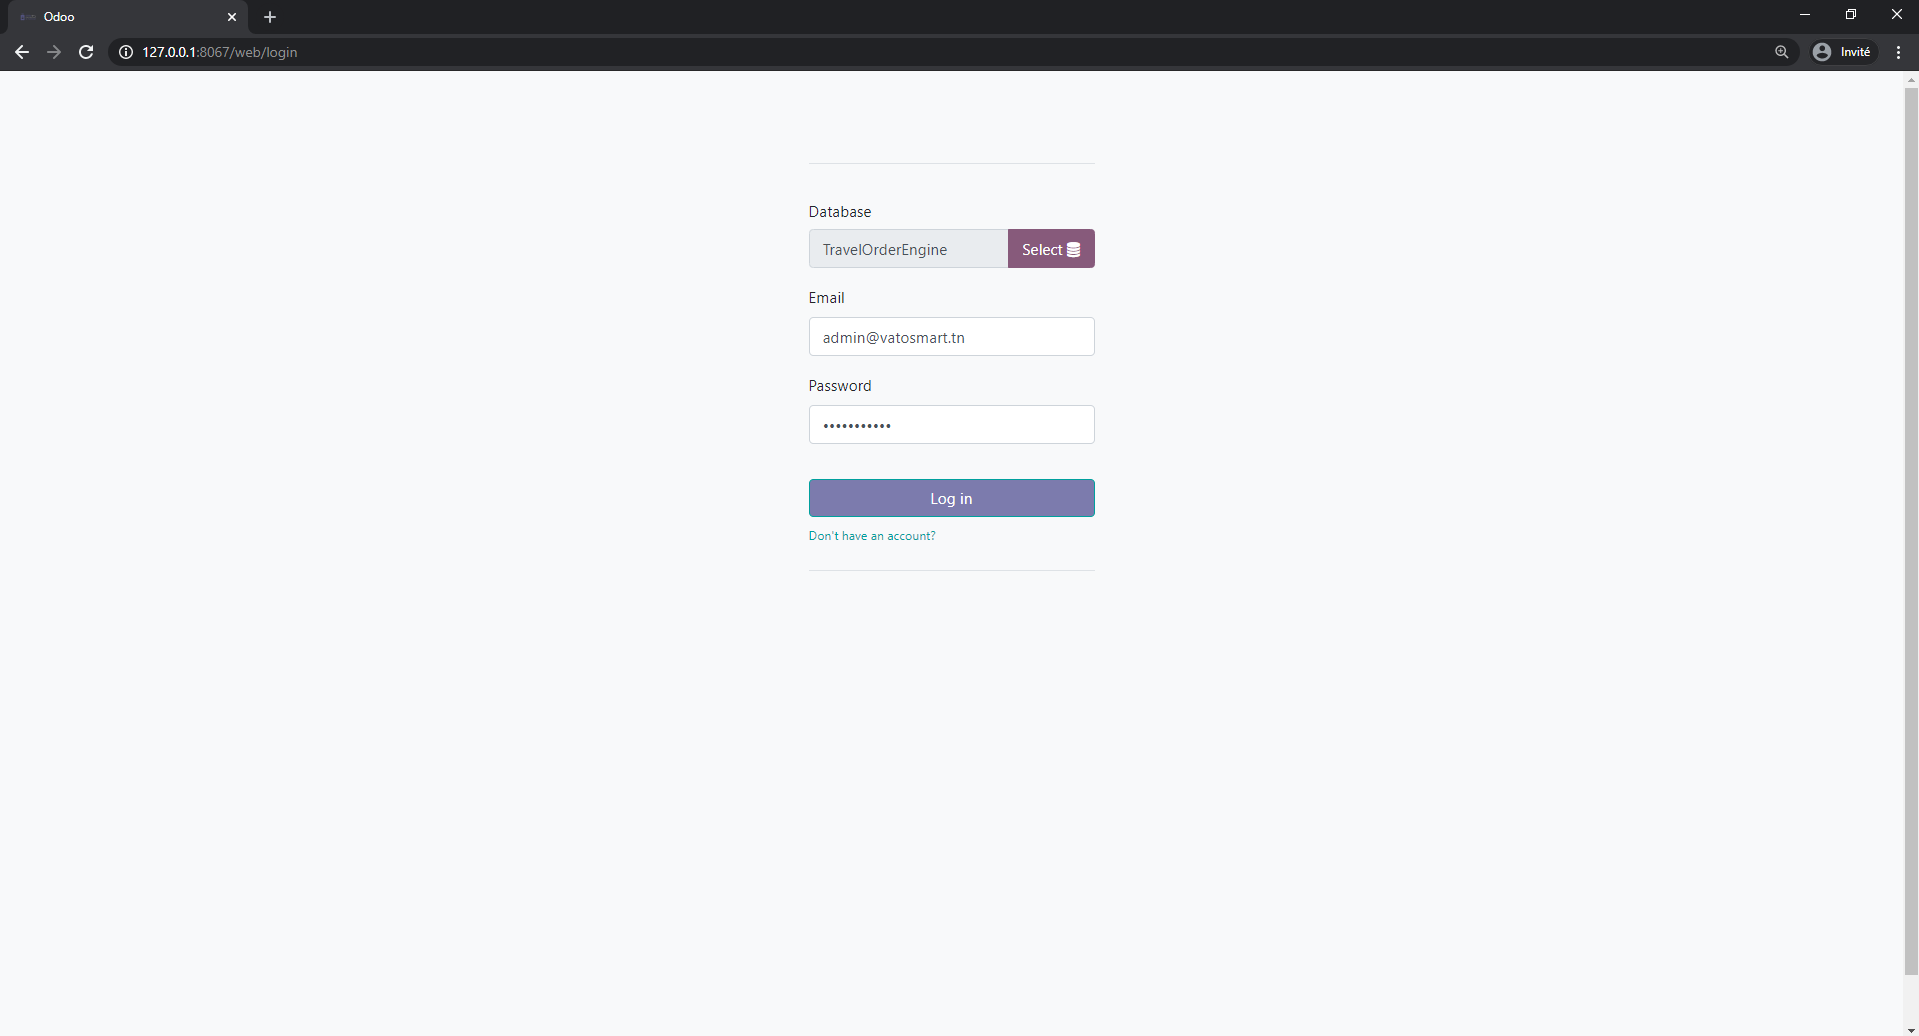
\includegraphics[scale=0.30]{img/c_auth.png}
    \caption{Interface <<Authentication>>}
    \label{fig:my_label}
\end{figure}

And on the next figure, we will show the main menu of this module, this navigation bar remains accessible from all views on this module.
\begin{figure}[H]
    \centering
    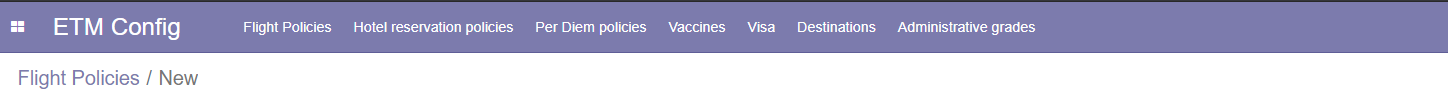
\includegraphics[scale=0.43]{img/c_config_menu.png}
    \caption{Configuration module menu}
    \label{fig:my_label}
\end{figure}
In this figure we will show the Countries list view, all countries are listed on this tree view and we can find our operations on the buttons above them. The administrator is the only actor able to access these views
\begin{figure}[H]
    \centering
    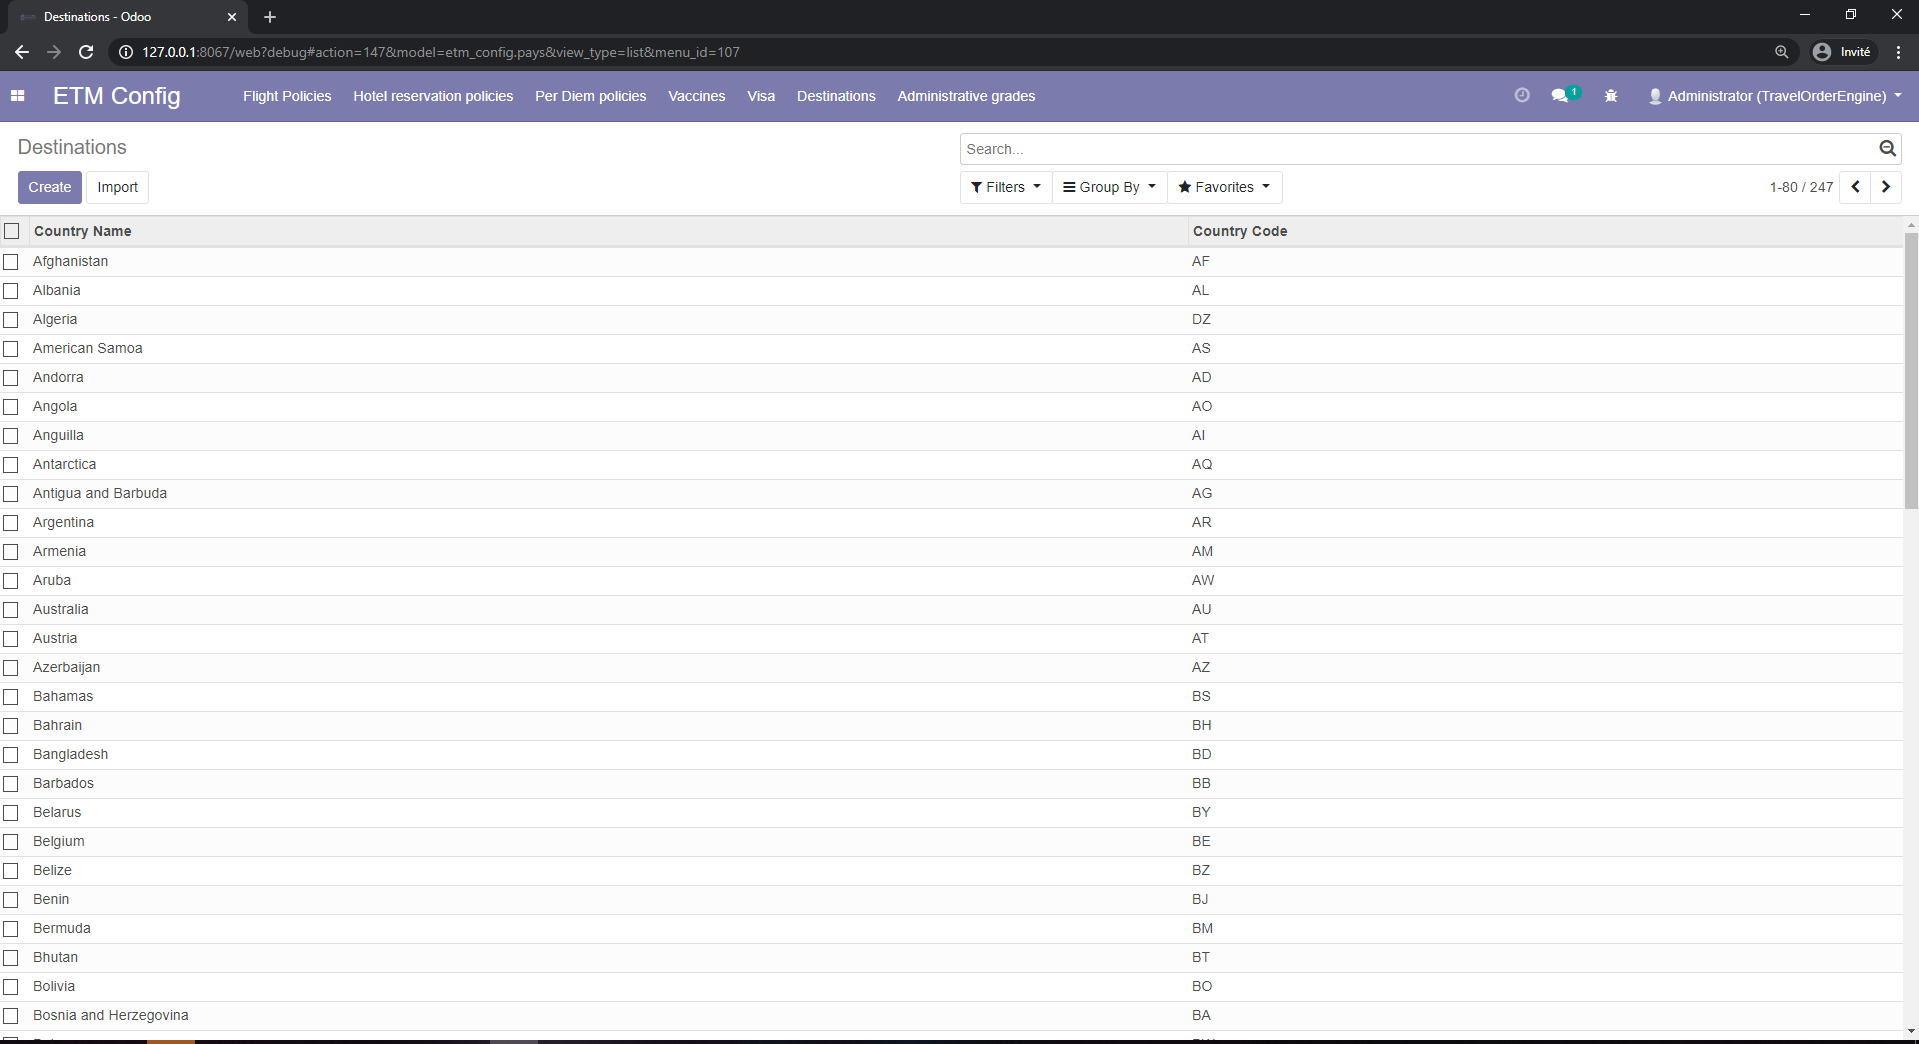
\includegraphics[scale=0.32]{img/c_country_list.png}
    \caption{Countries list view}
    \label{fig:my_label}
\end{figure}
In this figure we will go over the flight policy view, here we can Edit or Duplicate the policy we are viewing or we can create a new one
\begin{figure}[H]
    \centering
    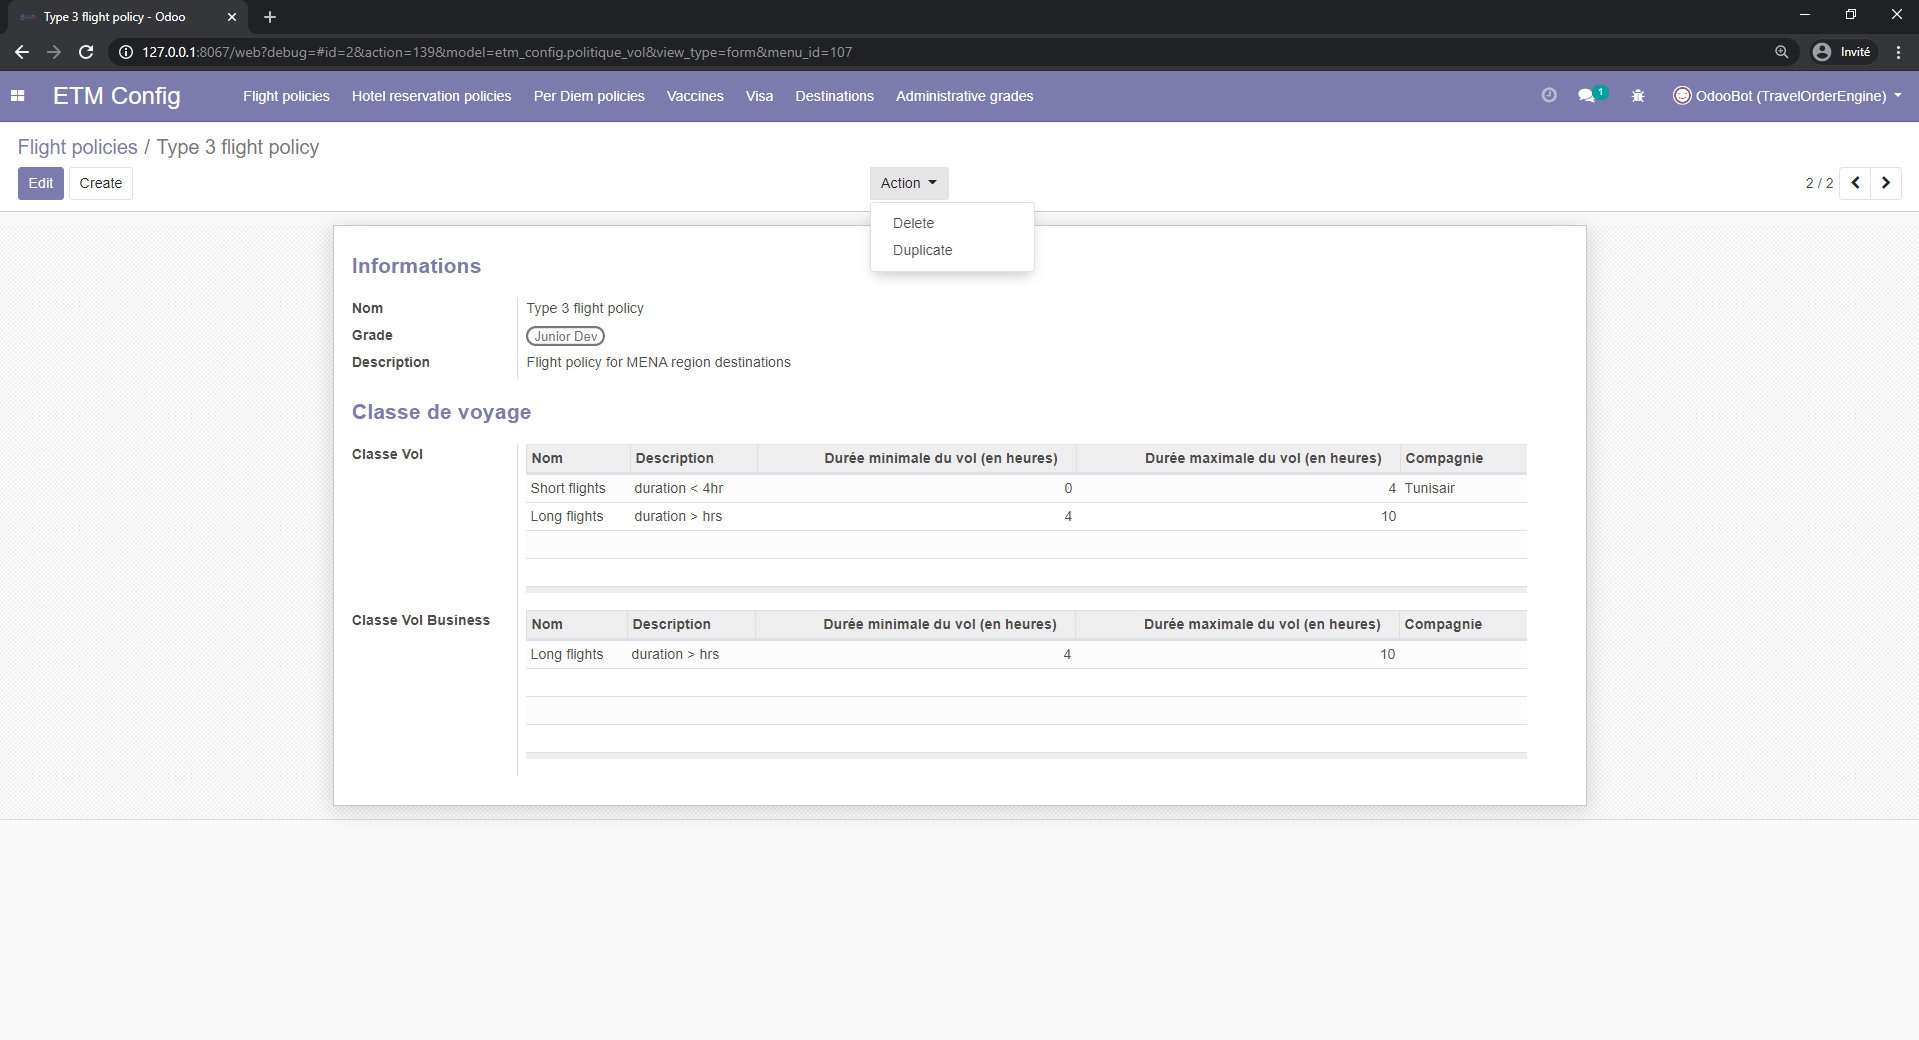
\includegraphics[scale=0.32]{img/c_flight_policy.png}
    \caption{Countries list view}
    \label{fig:my_label}
\end{figure}
\section*{Conclusion}
In this chapter we have discussed the sprint1 of our project which concerns the design, development and implementation of a first module our project which is the configuration module . This sprint was spread over one month. At the beginning of this sprint we set objectives to be reached. We started with the elaboration of the Backlog sprint afterwards we started a design phase before starting the development. \\During the development phase there was a daily meeting of the project working committee where everyone presented what they had done the day before, what they intended to do and if they faced any obstacles.\\ We closed this chapter with a section called realization where we presented some interfaces of the first increment of our project.\\
In what follows we will begin the second phase of the project, namely the design, development and implementation of a second module which concerns the management of Employees.

        \clearpage
        
        \chapter{Sprint 2}
	
\section*{Introduction}
   In this Sprint we go through the planning, analyzing, and implementing phases of the Employee module.\\
   At the beginning of this sprint, we held a second planning meeting where we set the following objectives:

\begin{itemize}
\item This sprint is spread over Three weeks.
\item At the end of this sprint the employee module will be delivered
\item Development of the sprint2 Backlog
\item Elaboration of a design phase
\end{itemize}
\\
This second iteration of our project's lifecycle encompasses the design, development and implementation of the Employee Managment module developed around the Odoo ERP base hr.employee model
\section{Sprint backlog}
The following table summarizes the tasks that we are responsible for carrying out 
\begin{center}
\begin{longtable}{|p{1cm}|p{6,25cm}|p{0,7cm}|p{6,25cm}|p{0,8cm}|}
\caption{ Project backlog }
\hline
\textbf{US ID} 
&\textbf{User Story}
&\textbf{T ID}
&\textbf{Task}
&\textbf{Esti- ma- tion}
\\
\hline
\multirow{ 3}{*}{0}
&\multirow{3}{*}{Storyless}
&0.1
&Class diagram
&4h\\\cline{3-5}
&
&0.2
&Use case diagram
&8h\\\cline{3-5}
&
&0.3
&Documenting progress
&2h\\\cline{3-5}
\hline
\multirow{2}{*}{2}
&\multirow{2}{=}{As an Administrator, I want to be able to create user accounts}
&2.1
&Create the «Employee» model
&8h\\\cline{3-5}
&
&2.2
&Link «Employee» model to Odoo user account
&8h\\\cline{3-5}

\hline
3
&As an Administrator, I want to be able to edit user details
&3.1
&Create «Employee» model security rules
&1h
\\\hline


\multirow{ 2}{*}{4}
&\multirow{2}{=}{As a Manager, I want to be able to edit user roles}
&4.1
&Define our user groups
&2h\\\cline{3-5}
&
&4.2
&Add the user groups to security file
&8h\\\cline{3-5}
\hline


\multirow{ 4}{*}{5}
&\multirow{4}{=}{As an Administrator, I want to be able to view the users list}
&5.1
&Create the «All Employees» view
&8h\\\cline{3-5}
&
&5.2
&Add search and filter actions
&4h\\\cline{3-5}
&
&5.3
&Create security rules
&1h\\\cline{3-5}
&
&5.4
&Create the «Users» menu item
&30m\\\cline{3-5}

\hline


\multirow{4}{*}{6}
&\multirow{4}{=}{As a User , I want to be able to view my profile details}
&6.1
&Create the «Employee» view
&16h\\\cline{3-5}
&
&6.2
&Create the «vaccine\_record» model
&4h\\\cline{3-5}
&
&6.3
&Create the «visa\_record» model
&4h\\\cline{3-5}
&
&6.4
&Add related models to the view
&6h\\\cline{3-5}

\hline

\multirow{2}{*}{7}
&\multirow{2}{=}{As a User , I want to be able to change my profile details}
&7.1
&Create model security rules
&1h\\\cline{3-5}
&
&7.2
&Change the editable attribute on desired fields
&2h\\\cline{3-5}

\hline
\end{longtable}
\end{center}
\section{Software Design}
The conceptual study conducted at the beginning of an iteration allows us to evaluate the sprint in its early stages by providing a stable reference of conceptual data model and processing to identify potential scenarios.

        \subsection{Use case diagram}
    \begin{figure}[H]
    \begin{center}
        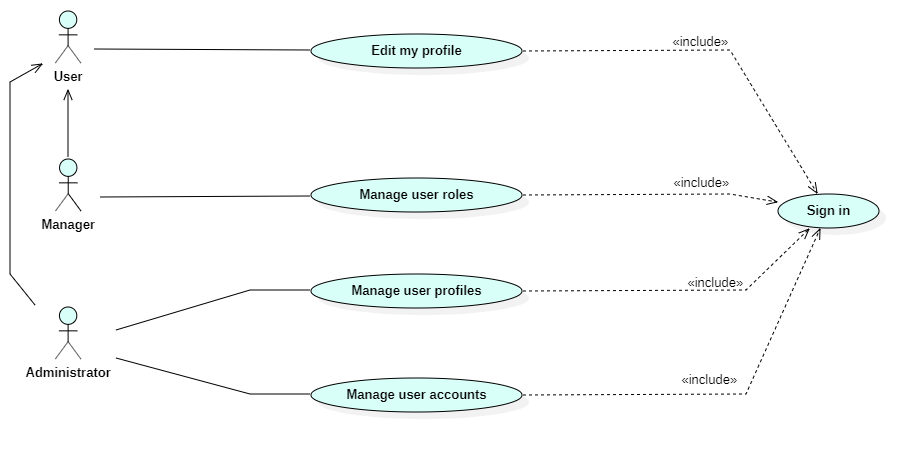
\includegraphics[scale=0.4]{img/sprint2_usecase.png}
        \caption{Sprint 2 use case diagram}
    \end{center}
     \label{fig:my_label}
\end{figure}

    \subsection{Class diagram}
        \begin{figure}[H]
    \begin{center}
        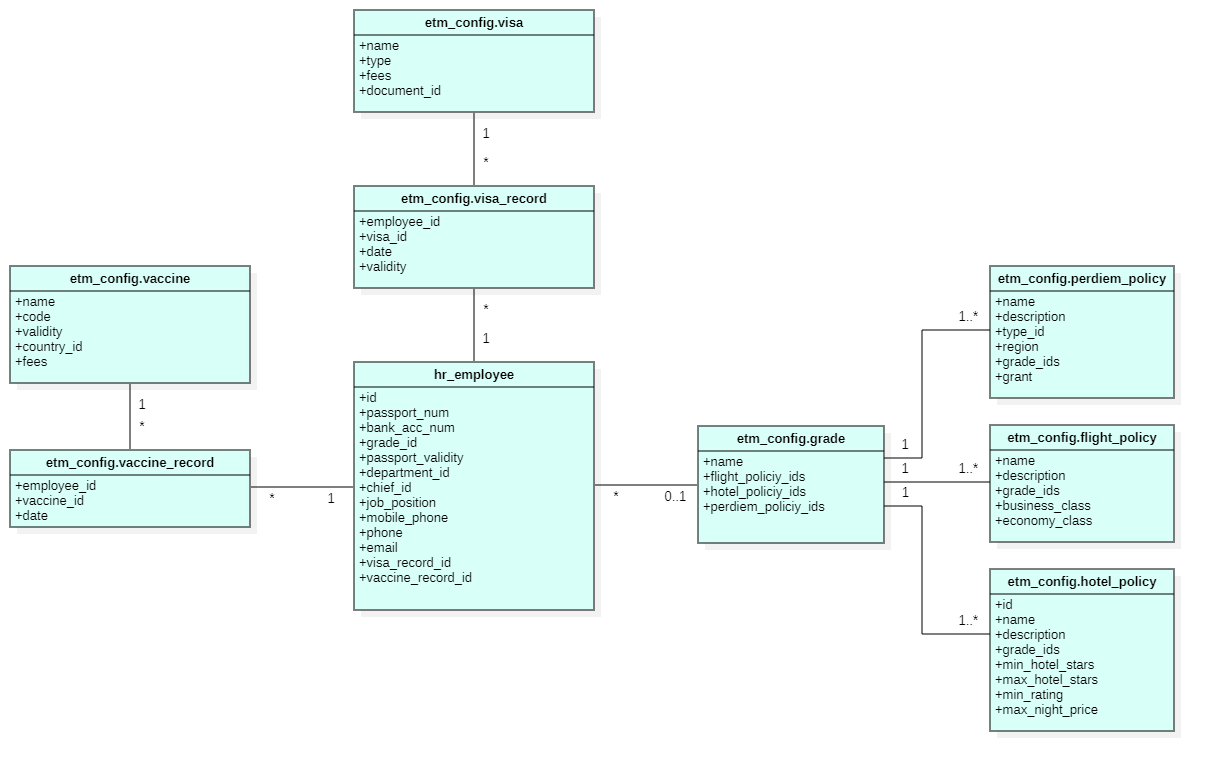
\includegraphics[scale=0.42]{img/sprint2_class.png}
        \caption{Sprint 2 class diagram}
    \end{center}
     \label{fig:my_label}
\end{figure}
        

In this section we will present the refinement of some use cases as well as the sequence diagram. 

\subsection*{Use case «Edit my profile»}
\begin{figure}[H]
    \begin{center}
        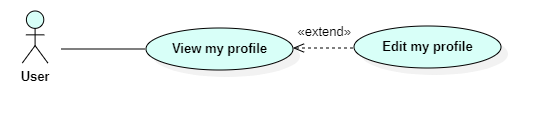
\includegraphics[scale=0.6]{img/sprint2_edit_profile_usecase.png}
        \caption{«Edit my profile» detailed use case diagram}
    \end{center}
        \label{fig:my_label}
\end{figure} 
    The following table addresses the use case previously illustrated by providing a textual description, post and preconditions as well as the main scenario and the nominal scenario
    \begin{center}
    
\begin{longtable}{|p{4,25cm}|p{9,25cm}|}
\caption{«Edit my profile» detailed textual description}
\hline
\textbf{Use Case}&Edit my profile
\\\hline
\textbf{Actors}&User
\hline
\textbf{Pre-condition}&User signed in and viewing profile
\hline
\textbf{Post-condition}&Profile edited
\hline
\textbf{Basic path}&
        \begin{enumerate}
         \item The user clicks on the button "Edit"
         \item The system displays a form containing current information
         \item The user edits the information
         \item The user clicks on the button "Save"
         \item The system processes the input
         \item The system saves the new information
         \item The user is sent back to the profile view
     \end{enumerate}\\
\hline
\textbf{Alternative path}&
\begin{itemize}
\item 4.Duplicate or missing Data (The user is sent back to step 2)
\item 4.No changes were made (The system skips to step 7)
\end{itemize}\\
\hline
\end{longtable}
\end{center}




\subsection*{Use case «Manage user roles»}
\begin{figure}[H]
    \begin{center}
        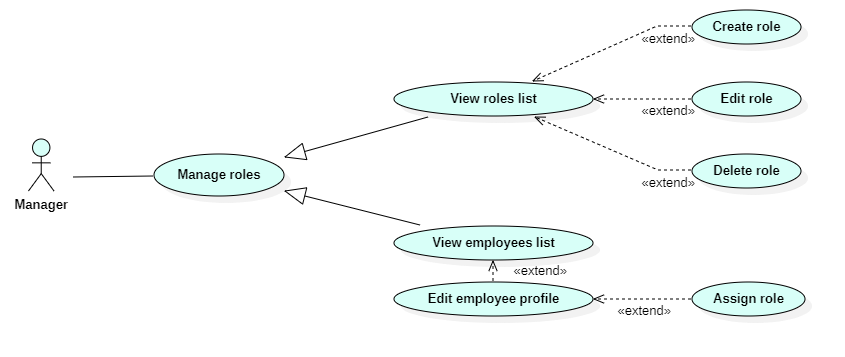
\includegraphics[scale=0.6]{img/sprint2_manage_roles_usecase.png}
        \caption{«Manage user roles» detailed use case diagram}
    \end{center}
        \label{fig:my_label}
\end{figure} 
    The following tables addresses the «Edit employee profile» use case detailing access and edit rights for each actor\\
    
\begin{center}
\begin{longtable}{|p{6,25cm}|p{1,5cm}|p{1,5cm}|p{1,5cm}|}
\caption{«User profile» access right}
\hline
&User&Manager&Admin
\\\hline
Can view user list&Yes&Yes&Yes
\hline
Can view user public information&Yes&Yes&Yes
\hline
Can view user private information&No&Yes&Yes
\hline
Can view user policies&No&Yes&Yes
\hline
Can view user Visa and vaccine history&No&Yes&Yes
\hline

\end{longtable}
\end{center}
\newpage
\begin{center}
\begin{longtable}{|p{6,25cm}|p{1,5cm}|p{1,5cm}|p{1,5cm}|}
\caption{«User profile» edit right}
\hline
&User&Manager&Admin
\hline
Can edit own profile&Yes&Yes&Yes
\hline
Can edit other's profile&No&Yes&Yes
\hline
Can edit other's private information&No&No&Yes
\hline
Can edit other's public information&No&No&Yes
\hline
Can assign policies&No&Yes&Yes
\hline
Can assign roles&No&Yes&Yes
\hline
Can edit visa and vaccine history&No&No&Yes
\hline
\end{longtable}
\end{center}





\subsection*{Use case «Manage user profiles»}
\begin{figure}[H]
    \begin{center}
        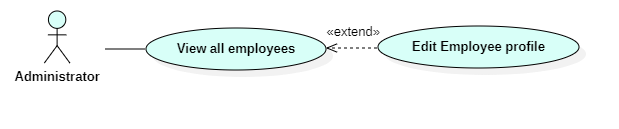
\includegraphics[scale=0.6]{img/sprint2_admin_edit_profile_usecase.png}
        \caption{«Manage user profiles» detailed use case diagram}
    \end{center}
        \label{fig:my_label}
\end{figure} 

The Administrator has the right to edit all fields of the user profile, these fields are split into categories. the table below will list all fields and their respective categories:\\
\newpage
\begin{center}
\begin{longtable}{|p{4,25cm}|p{9,25cm}|}
\caption{«Employee profile» fields list}
\hline
\textbf{Public information}&
\begin{itemize}
\item Full name
\item Phone
\item Mobile phone
\item Department
\item Job Position
\item Hierarchical Chief
\end{itemize}
\hline
\textbf{Private information}&
\begin{itemize}
\item Identifier
\item Bank account number
\item Passport number
\item Passport validity
\end{itemize}
\hline
\textbf{Policies}&
\begin{itemize}
\item Flight policy
\item Hotel reservation policy
\item Per Diem policy
\end{itemize}
\hline
\textbf{Grade}&Grade
\hline
\end{longtable}
\end{center}



\subsection*{Use case «Manage user accounts»}
\begin{figure}[H]
    \begin{center}
        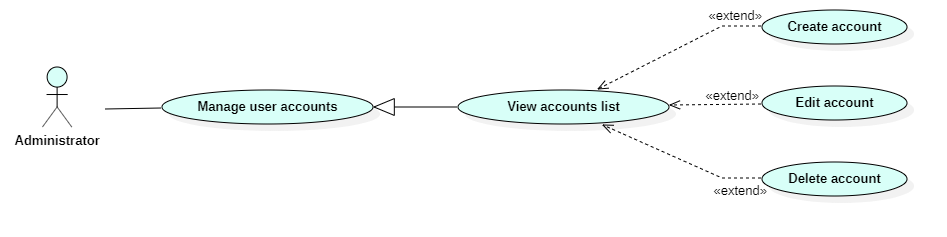
\includegraphics[scale=0.55]{img/sprint2_manage_accounts_usecase.png}
        \caption{«Manage user accounts» detailed use case diagram}
    \end{center}
        \label{fig:my_label}
\end{figure} 

\begin{center}
\begin{longtable}{|p{4,25cm}|p{9,25cm}|}
\caption{«Create account» detailed textual description}
\hline
\textbf{Use Case}&Create account
\\\hline
\textbf{Actors}&Administrator
\hline
\textbf{Pre-condition}&Administrator signed in and viewing account list
\hline
\textbf{Post-condition}&Account created
\hline
\textbf{Basic path}&
        \begin{enumerate}
         \item The Administrator clicks on the button "Create"
         \item The system displays a a empty form
         \item The Administrator fills the form
         \item The Administrator clicks on the button "Save"
         \item The system processes the input
         \item The system creates a new account
         \item The Administrator is sent back to the account list view
     \end{enumerate}\\
\hline
\textbf{Alternative path}&
\begin{itemize}
\item 4.Duplicate or missing Data (The Administrator is sent back to step 2)
\item 2.Administrator clicks on the button "Cancel"(System skips to step 7)
\end{itemize}\\
\hline
\end{longtable}
\end{center}



\section{Implementation}
This section presents some user interfaces of the module with screenshots to further clarify our work. The figures below present these interfaces, starting with the first figure which shows the Employee list view , in this view we can access any employee file or create new employees

\begin{figure}[H]
    \centering
    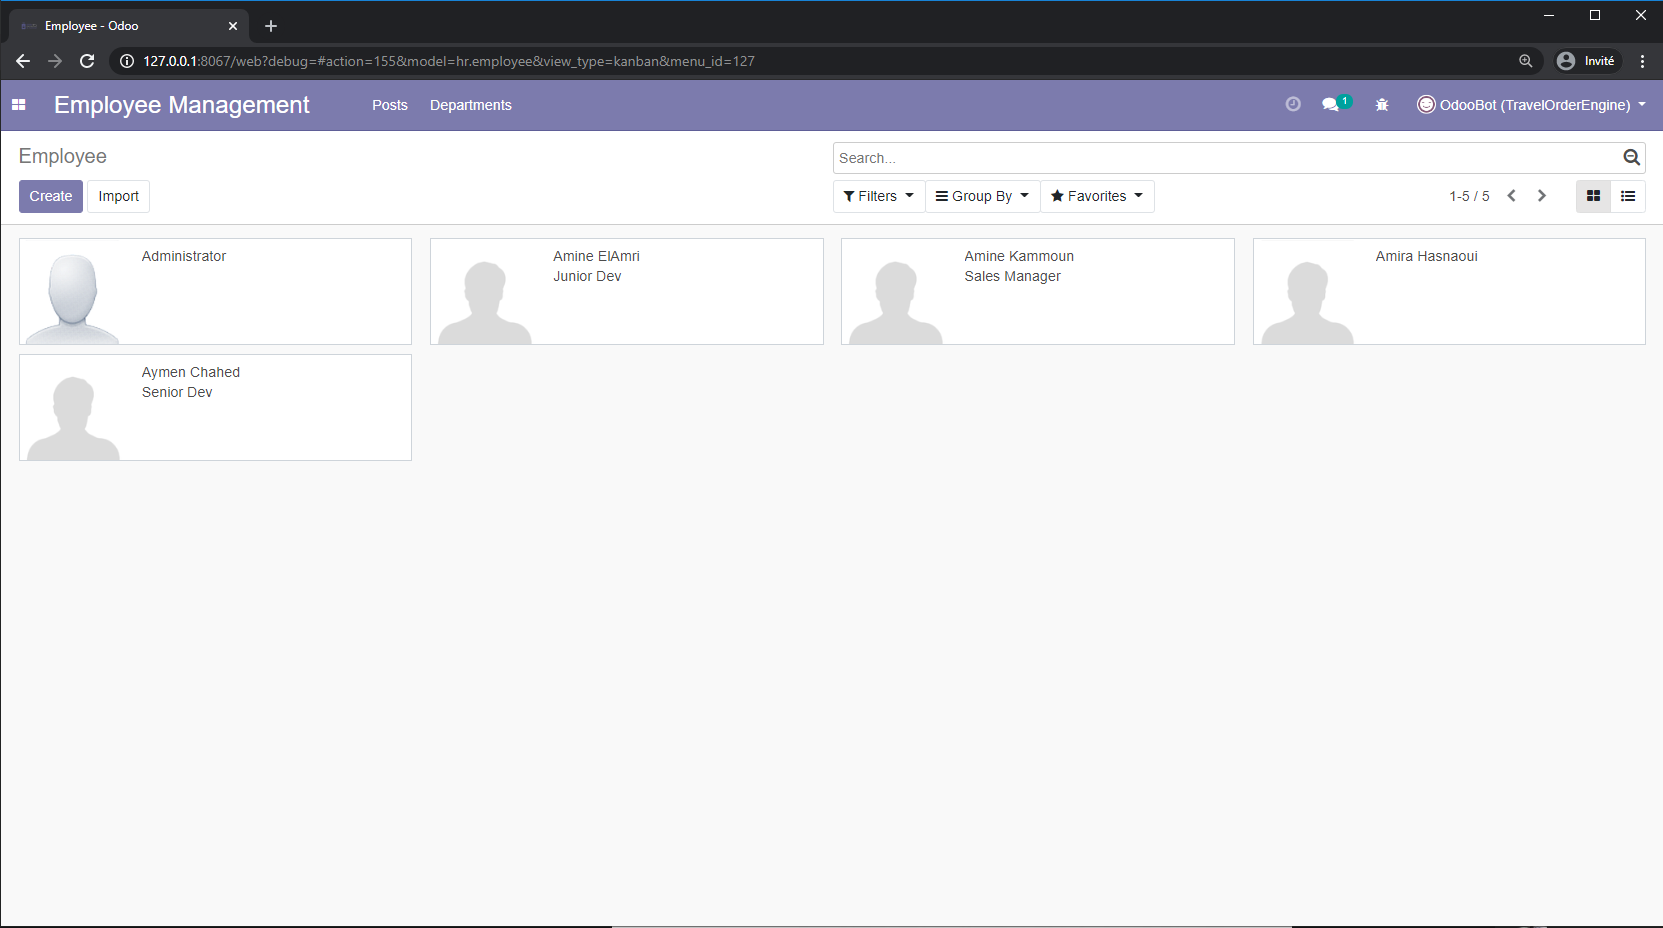
\includegraphics[scale=0.38]{img/c_employees.png}
    \caption{Employees list view}
    \label{fig:my_label}
\end{figure}

In this figure we will show the Employee view, All the employee information is displayed here . it is the same form we use for creating employees. The administrator can edit all the information by clicking the "Edit" button above
\begin{figure}[H]
    \centering
    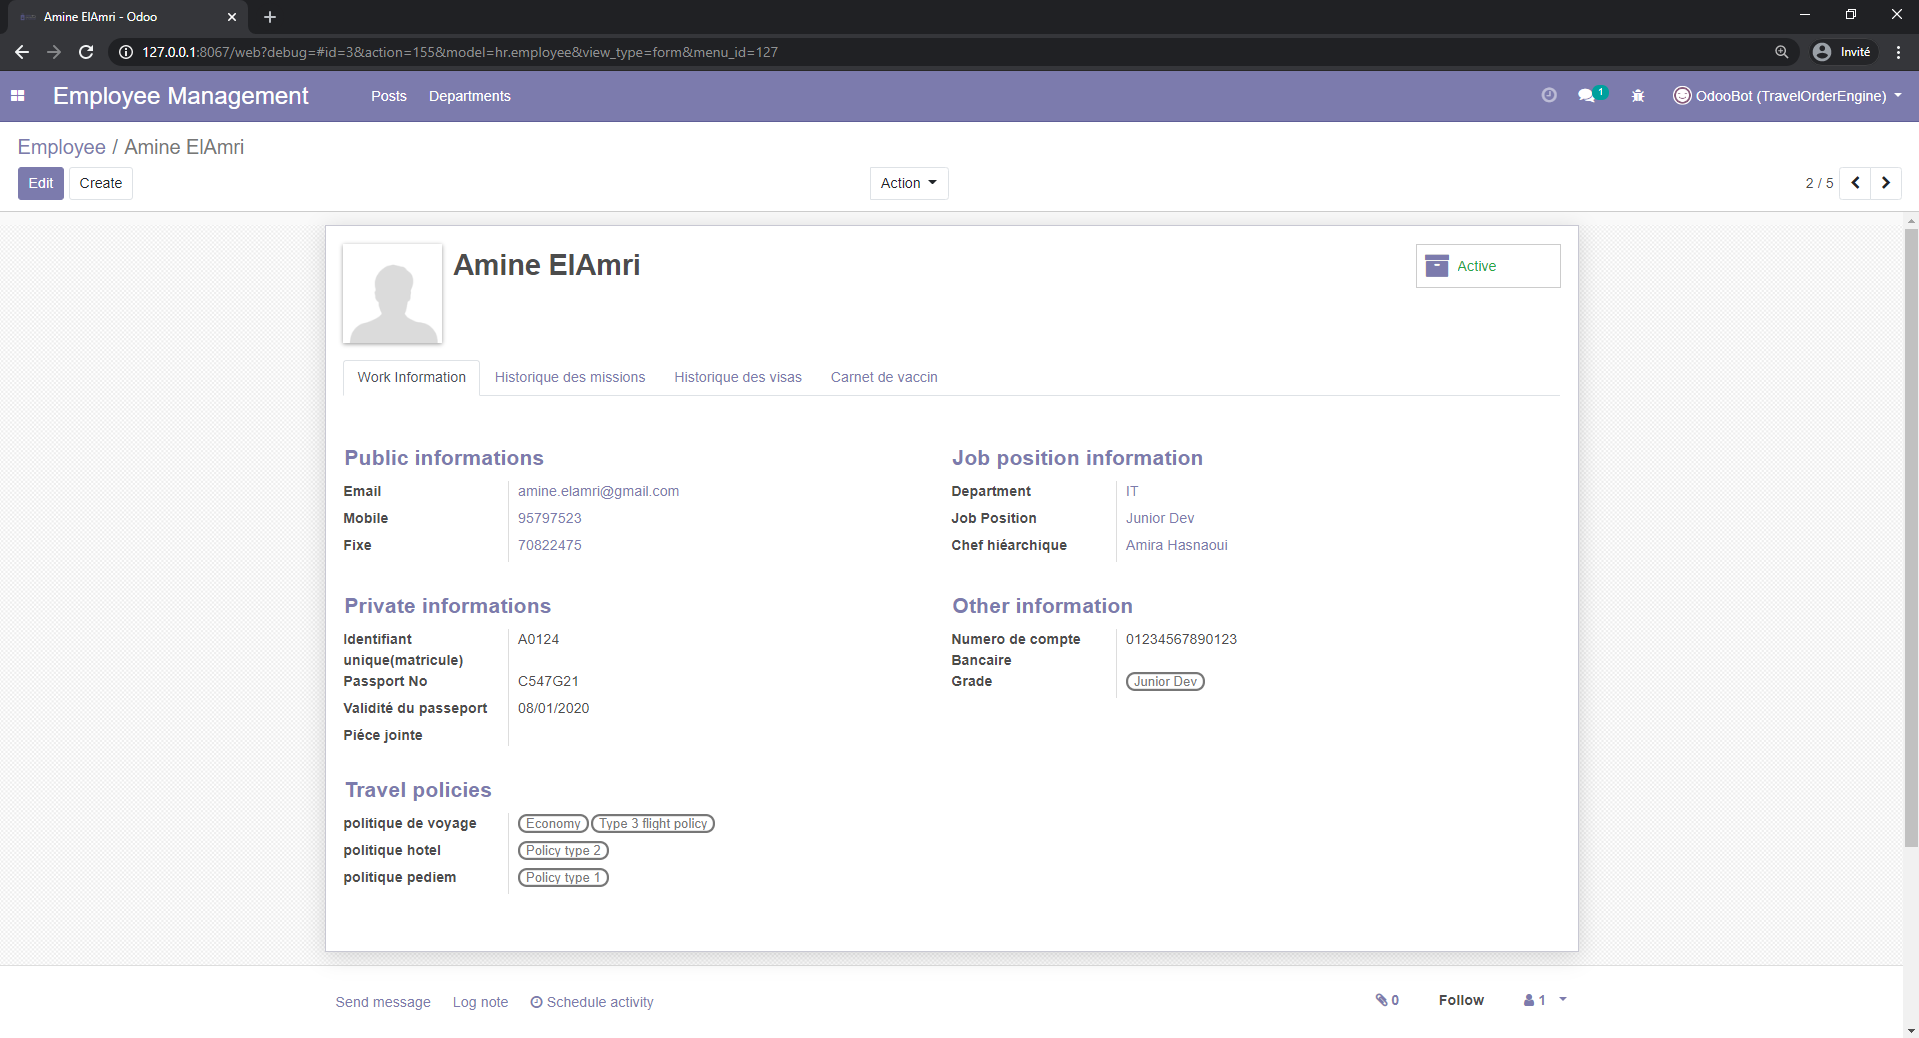
\includegraphics[scale=0.33]{img/c_employee.png}
    \caption{Employee view}
    \label{fig:my_label}
\end{figure}
In this figure we will show the Department list view, here we can create and edit the departments and set the department's manager.
\begin{figure}[H]
    \centering
    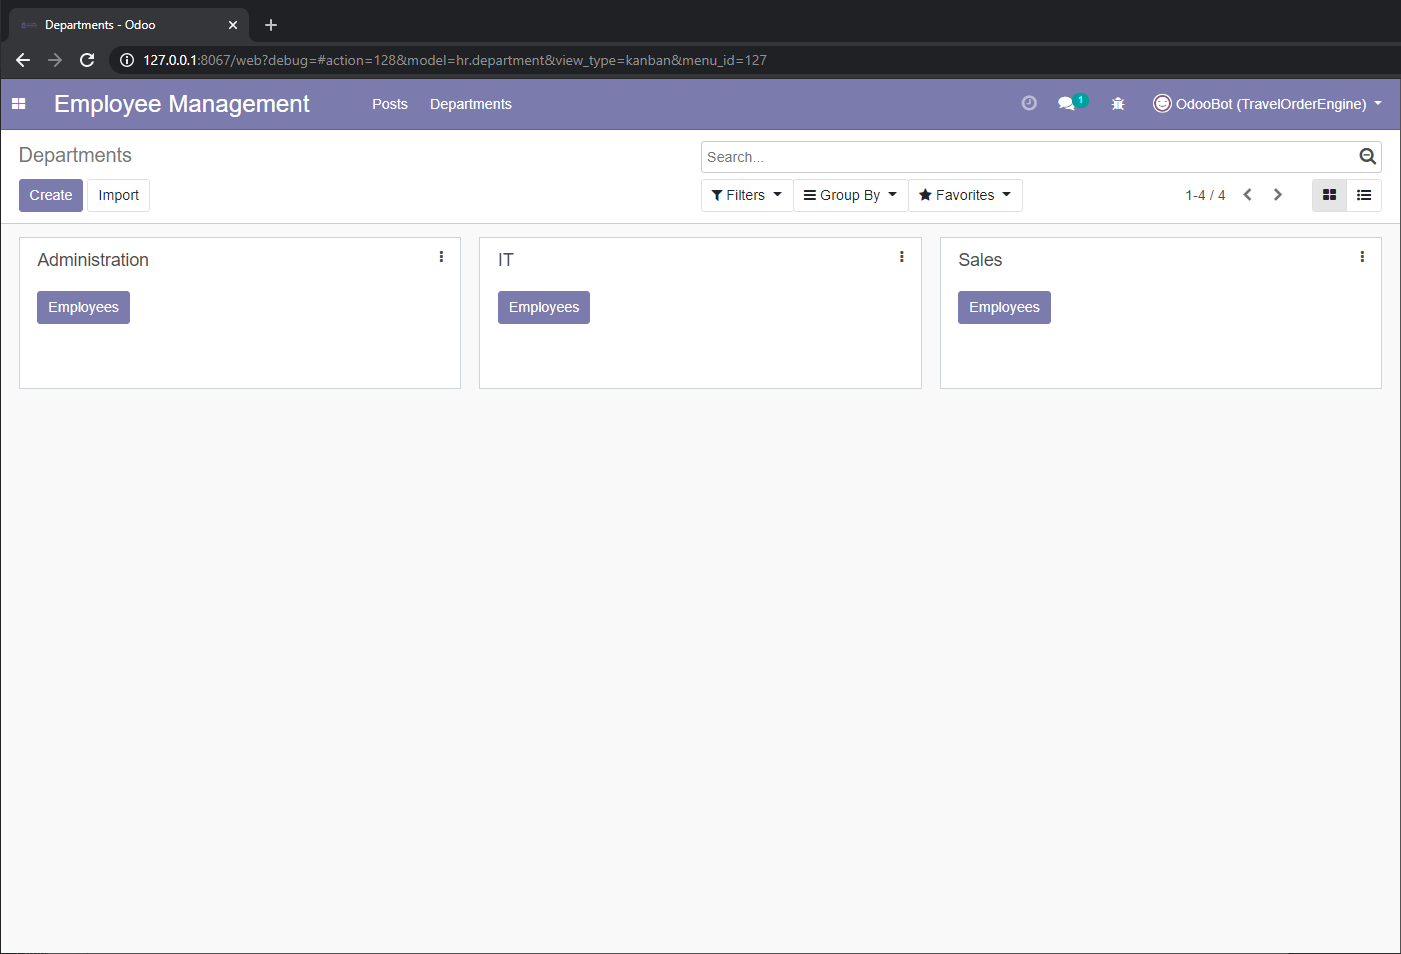
\includegraphics[scale=0.44]{img/c_departements.png}
    \caption{Departments list view}
    \label{fig:my_label}
\end{figure}
In this last figure we will show the job positions list view , Administrator can add or edit jobs on this list, Employees can have only 1 job position at a time.
\begin{figure}[H]
    \centering
    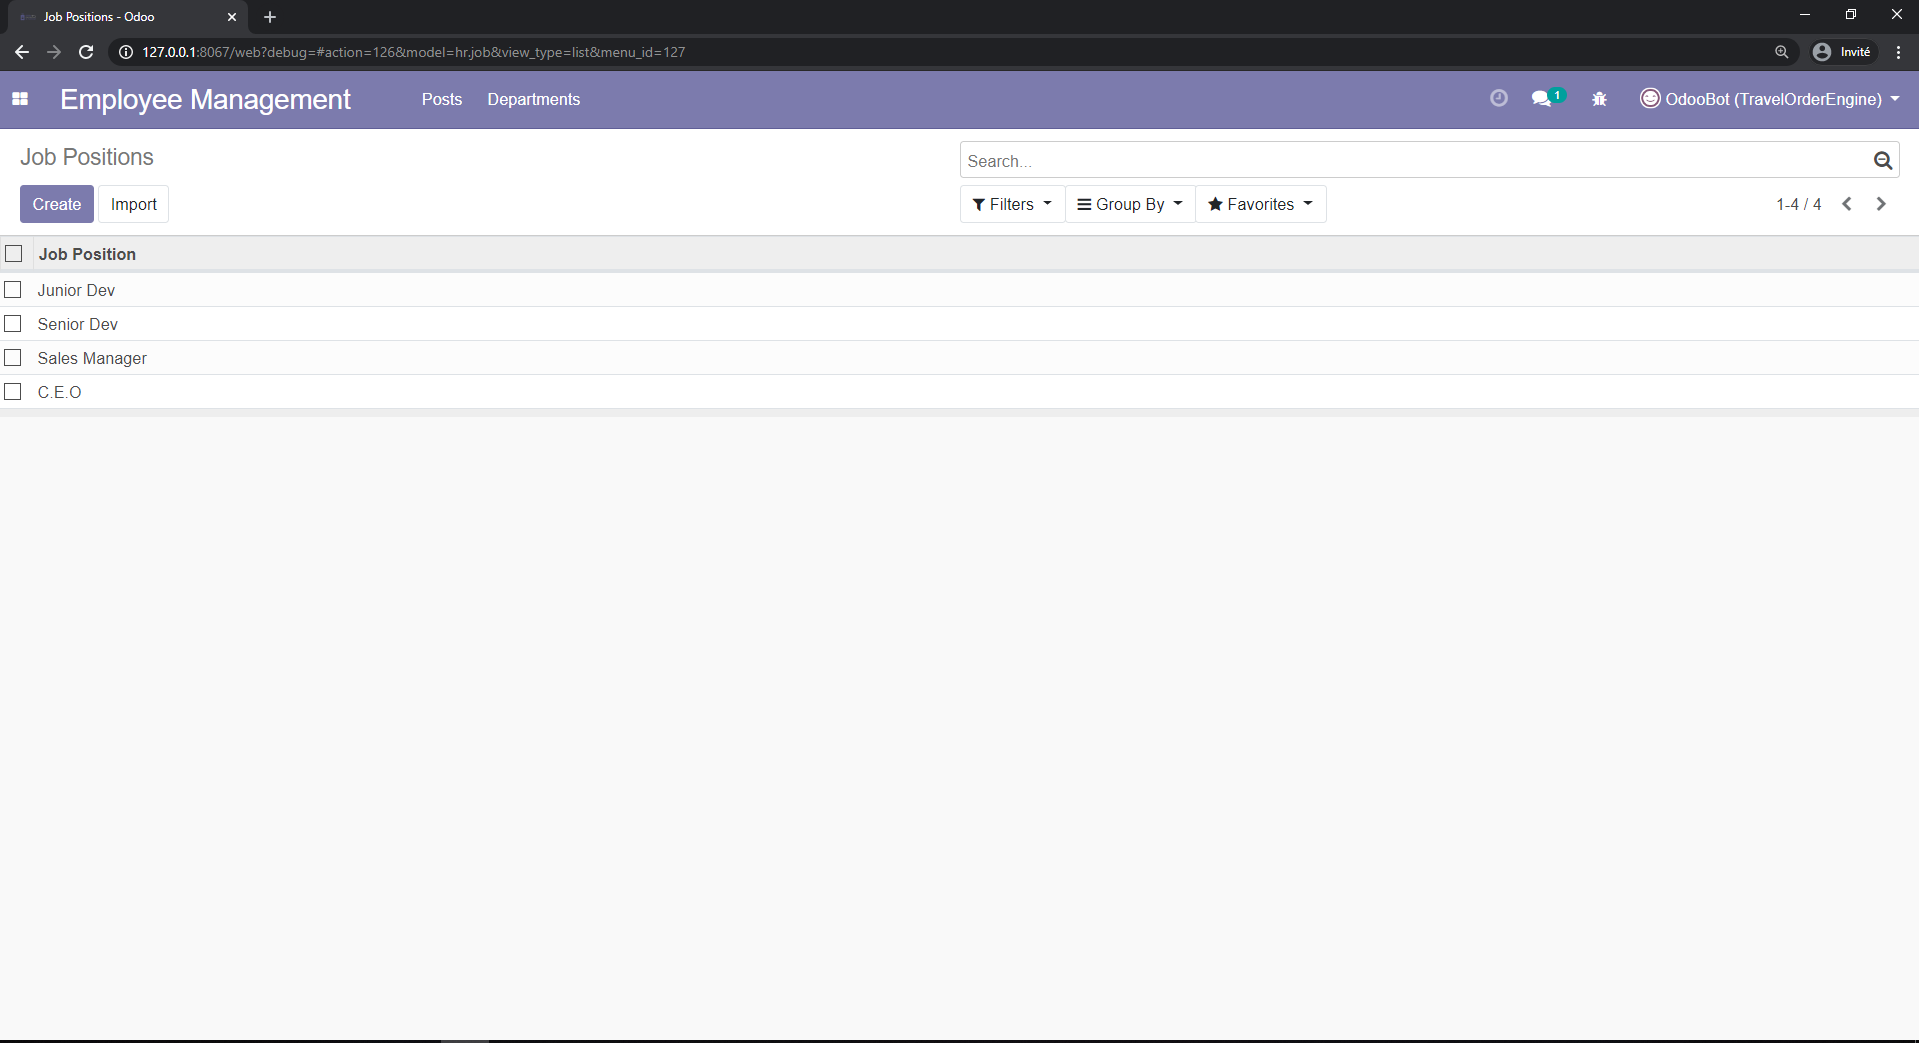
\includegraphics[scale=0.32]{img/c_jobs.png}
    \caption{Job positions list view}
    \label{fig:my_label}
\end{figure}





\section*{Conclusion}
  This chapter covered the sprint2 of our project. We started by explaining the objective of this sprint and the main actors. Then we presented our Sprint2 backlog. We continued with the design phase where we schematized some design diagrams in UML and we closed the chapter by exposing the interfaces of the second increment.  \\ 
In the following, we will address the last sprint of this project which will involve the design, development, and implementation of the travel order management module.
        \clearpage
        
        \chapter{Sprint 3}
	
\section*{Introduction}
    The third sprint of the project's life cycle started on a team-wide planning meeting and resulted in the following:
    \begin{itemize}
        \item This sprint is spread out over five weeks
        \item  At the end of this sprint, the Travel order module will be delivered as well as the first release of the project. 
        \item Development of the sprint 3 Backlog
        \item Elaboration of a design phase
    \end{itemize}
\subsection*{Purpose of the module}
This module is the main module of our project, In this module, the travel order is created, processed, and closed. Each of the actors has his role in this module but it all boils down to basic workflow.
\subsection*{Actors}
\begin{itemize}
\item \textbf{User}: Creates and manages his travel orders.
\item \textbf{Manager}: Confirms draft and validates agents' work.
\item \textbf{Agent}: Process the travel orders
\end{itemize}
\subsection*{Travel order phases}
The figure below shows all the order states in the workflow.
\begin{figure}[H]
    \begin{center}
        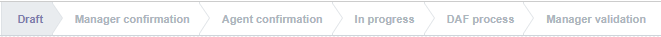
\includegraphics[scale=0.9]{img/workflow.png}
        \caption{travel order workflow}
    \end{center}
        \label{fig:my_label}
\end{figure} 
And in this flowchart diagram we go over them:
    \begin{center}
        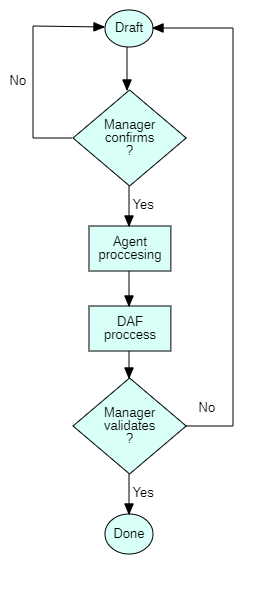
\includegraphics[scale=0.6]{img/workflow2.png}
        \caption{travel order flowchart diagram}
    \end{center}
\section{Sprint backlog}
The following table summarizes the tasks that we are responsible for carrying out 
\begin{center}
\begin{longtable}{|p{1cm}|p{6,25cm}|p{0,7cm}|p{6,25cm}|p{0,8cm}|}
\caption{ Project backlog }
\hline
\textbf{US ID} 
&\textbf{User Story}
&\textbf{T ID}
&\textbf{Task}
&\textbf{Esti- ma- tion}
\\
\hline
\multirow{ 3}{*}{0}
&\multirow{3}{*}{Storyless}
&0.1
&Class diagram
&4h\\\cline{3-5}
&
&0.2
&Use case diagram
&8h\\\cline{3-5}
&
&0.3
&Documenting progress
&2h\\\cline{3-5}
\hline

\multirow{2}{*}{19}
&\multirow{2}{=}{As a User , I want to be able to create, edit and delete travel order drafts}
&19.1
&Create the «Mission» model
&8h\\\cline{3-5}
&
&19.2
&Create the «Mission\_form» view
&2h\\\cline{3-5}
&
&19.3
&Create the security rules
&30m\\\cline{3-5}

\hline


\multirow{ 2}{*}{20}
&\multirow{2}{=}{As a User , I want to be able to see all my travel orders}
&20.1
&Create the «ETM Mission» menu
&30m\\\cline{3-5}
&
&20.2
&Create the «My Orders» menu item
&30m\\\cline{3-5}
&
&20.3
&Create the «User\_Dashboard» view
&4h\\\cline{3-5}
\hline


\multirow{2}{*}{21}
&\multirow{2}{=}{As a User , I want to be able to filter my travel orders by status or date}
&21.1
&Add status filter to the «User\_Dashboard» view
&4h\\\cline{3-5}
&
&21.2
&Add date filter to the «User\_Dashboard» view
&4h\\\cline{3-5}

\hline

\multirow{3}{*}{22}
&\multirow{3}{=}{As a User , I want to be able to file my travel order drafts and track their progress}
&22.1
&Create the «workflow.xml» view
&8h\\\cline{3-5}
&
&22.2
&Add  «Confirm» action to the draft view
&2h\\\cline{3-5}
&
&22.3
&Add status indicator to the «User\_Dashboard» view
&2h\\\cline{3-5}

\hline

23
&As an Agent , I want to be able to see all travel orders
&23.1
&Create the «Agent\_Dashboard» view
&8h\\\cline{3-5}

\hline

\multirow{2}{*}{24}
&\multirow{2}{=}{As an Agent , I want to be able to add attachments to travel orders}
&24.1
&Create the «Add\_Attachments» widget
&6h\\\cline{3-5}
&
&24.2
&Create attachment constraints and verification
&2h\\\cline{3-5}
\hline

\multirow{2}{*}{25}
&\multirow{2}{=}{As an Agent , I want to be able to change travel orders’ status}
&25.1
&Add «Agent\_confirm» action to the workflow
&4h\\\cline{3-5}
&
&25.2
&Add «Agent\_deny» action to the workflow
&4h\\\cline{3-5}
\hline

\multirow{2}{*}{26}
&\multirow{2}{=}{As a Manager , I want to be able to see all travel orders pending my confirmation}
&26.1
&Create the «Manager\_Dashboard» view
&6h\\\cline{3-5}
&
&26.2
&Add menu item «Management» to main menu
&30m\\\cline{3-5}
\hline

\multirow{2}{*}{27}
&\multirow{2}{=}{As a Manager , I want to be able to confirm or reject travel orders pending my confirmation}
&27.1
&Add «Manager\_confirm» action to the workflow
&4h\\\cline{3-5}
&
&27.2
&Add «Manager\_deny» action to the workflow
&4h\\\cline{3-5}
\hline


\end{longtable}
\end{center}


\section{Software Design}
Like the previous iterations we elaborate a conceptual study or we use UML diagrams to have a more in-depth view on the module.
    
         \subsection{Use case diagram}
    \begin{figure}[H]
    \begin{center}
        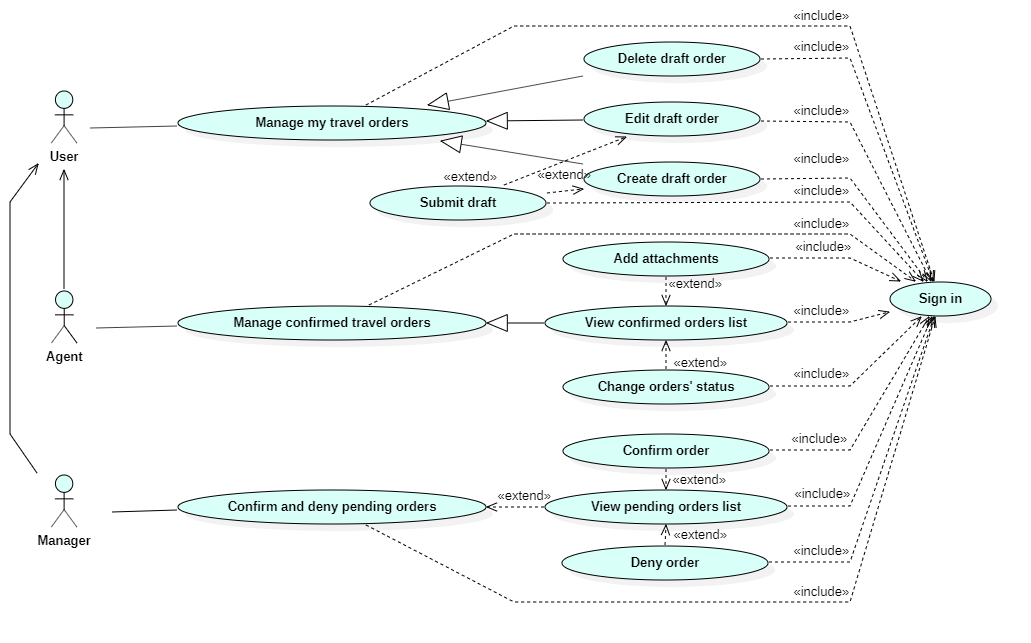
\includegraphics[scale=0.5]{img/sprint3_usecase.png}
        \caption{Sprint 3 use case diagram}
    \end{center}
     \label{fig:my_label}
\end{figure}
         \subsection{Class diagram}
    \begin{figure}[H]
    \begin{center}
        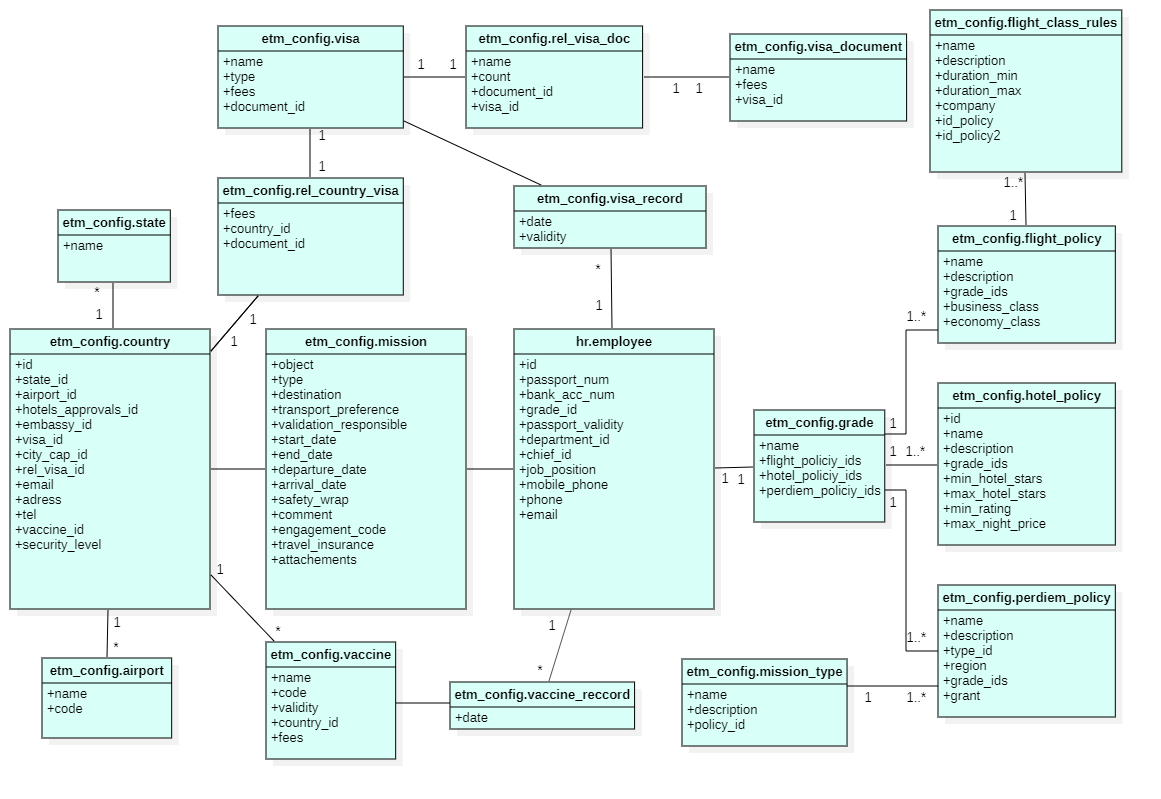
\includegraphics[scale=0.450]{img/sprint3_class.png}
        \caption{Sprint 3 class diagram}
    \end{center}
     \label{fig:my_label}
\end{figure}

In what follows, we will proceed to go in detail on some use cases\\
\subsection*{Use case «Manage my travel orders»}
\begin{figure}[H]
    \begin{center}
        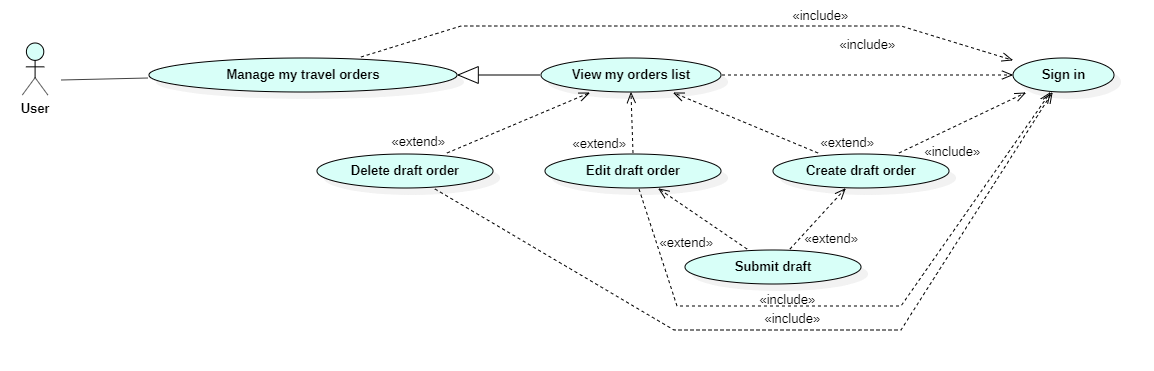
\includegraphics[scale=0.44]{img/sprint3_user_manage_usecase.png}
        \caption{«Manage my travel orders» detailed use case diagram}
    \end{center}
        \label{fig:my_label}
\end{figure} 
The User has the right to create new travel orders at any given time.\\
The User can only edit or delete travel orders that are currently in the "draft" phase.\\
The User can submit a draft order for his superiors to review and process. This order is no longer a draft and is now "pending confirmation"

\begin{center}
\begin{longtable}{|p{4,25cm}|p{9,25cm}|}
\caption{«Create draft order» detailed textual description}
\hline
\textbf{Use Case}&Create draft order
\\\hline
\textbf{Actors}&User
\hline
\textbf{Pre-condition}&User signed in and viewing his orders list
\hline
\textbf{Post-condition}&New draft travel order created
\hline
\textbf{Basic path}&
        \begin{enumerate}
         \item The User clicks on the button "New"
         \item The system displays a a empty form
         \item The User fills the form
         \item The User clicks on the button "Save"
         \item The System processes the input
         \item The System creates a new draft order
         \item The User is sent back to the orders list
     \end{enumerate}\\
\hline
\textbf{Alternative path}&
\begin{itemize}
\item 4.Duplicate or missing Data (The Administrator is sent back to step 2)
\item 2.User clicks on the button "Cancel"(System skips to step 7)
\end{itemize}\\
\hline
\end{longtable}
\end{center}



\subsection*{Use case «Manage confirmed travel orders»}
\begin{figure}[H]
    \begin{center}
        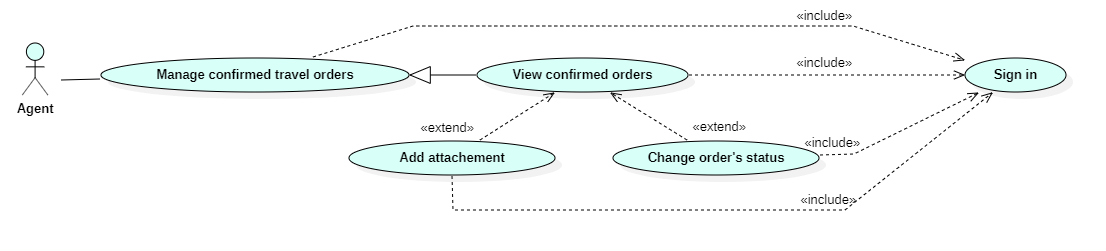
\includegraphics[scale=0.44]{img/sprint3_manage_confirmed_usecase.png}
        \caption{«Manage confirmed travel orders» detailed use case diagram}
    \end{center}
        \label{fig:my_label}
\end{figure} 

The Agent can only process travel orders that the Managers approved.\\
The process is split into 2 main parts :\\
\begin{itemize}
\item Adding attachments (reservations, visa documents, insurance ...)
\item Changing status (ToDo, in progress, Done)
\end{itemize}
\subsubsection*{«Add attachement» sequance diagram}
\begin{figure}[H]
    \begin{center}
        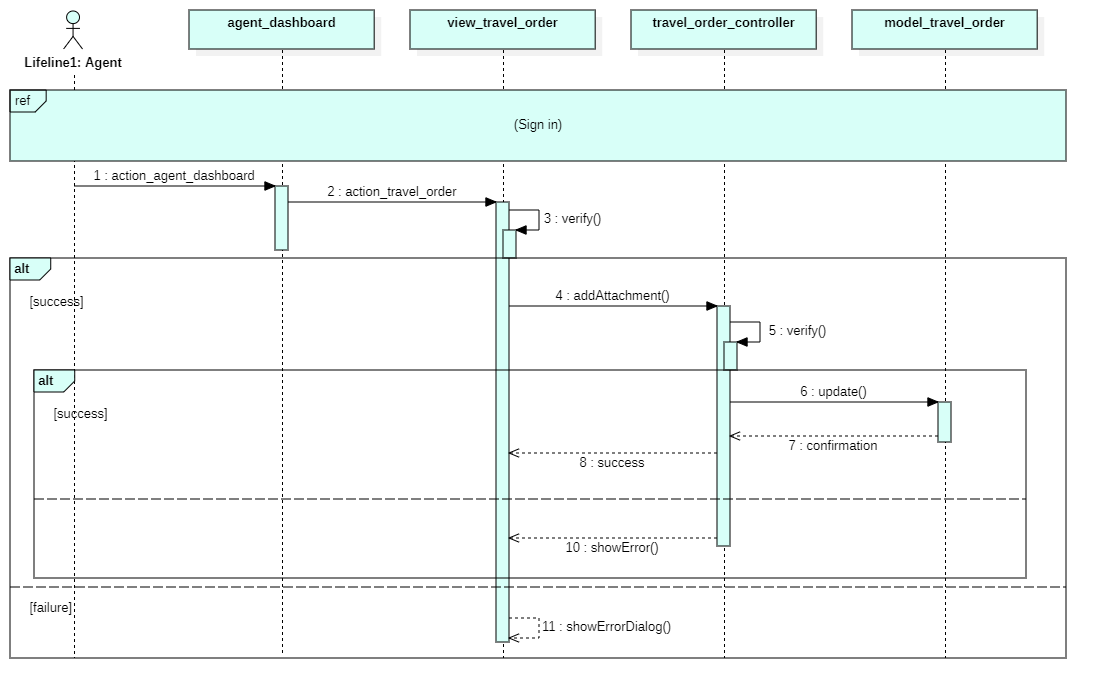
\includegraphics[scale=0.40]{img/sprint3_attach_sequ.png}
        \caption{«Manage confirmed travel orders» detailed use case diagram}
    \end{center}
        \label{fig:my_label}
\end{figure} 

\subsubsection*{Change status textual description}

\begin{center}
\begin{longtable}{|p{4,25cm}|p{9,25cm}|}
\caption{«Create draft order» detailed textual description}
\hline
\textbf{Use Case}&Change order status
\\\hline
\textbf{Actors}&Agent
\hline
\textbf{Pre-condition}&Agent signed in and viewing his dashboard
\hline
\textbf{Post-condition}&order status changed
\hline
\textbf{Basic path}&
        \begin{enumerate}
         \item The Agent drags the travel order card
         \item The Agent drops the card on one of the 3 zones
         \item The System changes the travel order status
     \end{enumerate}\\
\hline
\textbf{Alternative path}&
\begin{itemize}
\item 2.Agent drops the card outside the allocated space (back to step 1)
\item 2.Agent drops a unfinished order card on the "Done" section (back to step1)
\end{itemize}\\
\hline
\end{longtable}
\end{center}




\section{Implementation}
This section presents some user interfaces of the module with screenshots to further clarify our work. The figures below present these interfaces, starting with the first figure which shows the travel order draft. This view is the employee's interface.\\
All employee information is automatically generated and is not editable.\\
All policies are automatically generated (depending on the employee grade and destinations) and are not editable.\\
All Visas and Vaccines are automatically generated (depending on the destinations) and the employee can only change if he have them already or needs to obtain them by checking the checkbox.\\
The Employee can submit this draft by clicking the button above.

\begin{figure}[H]
    \centering
    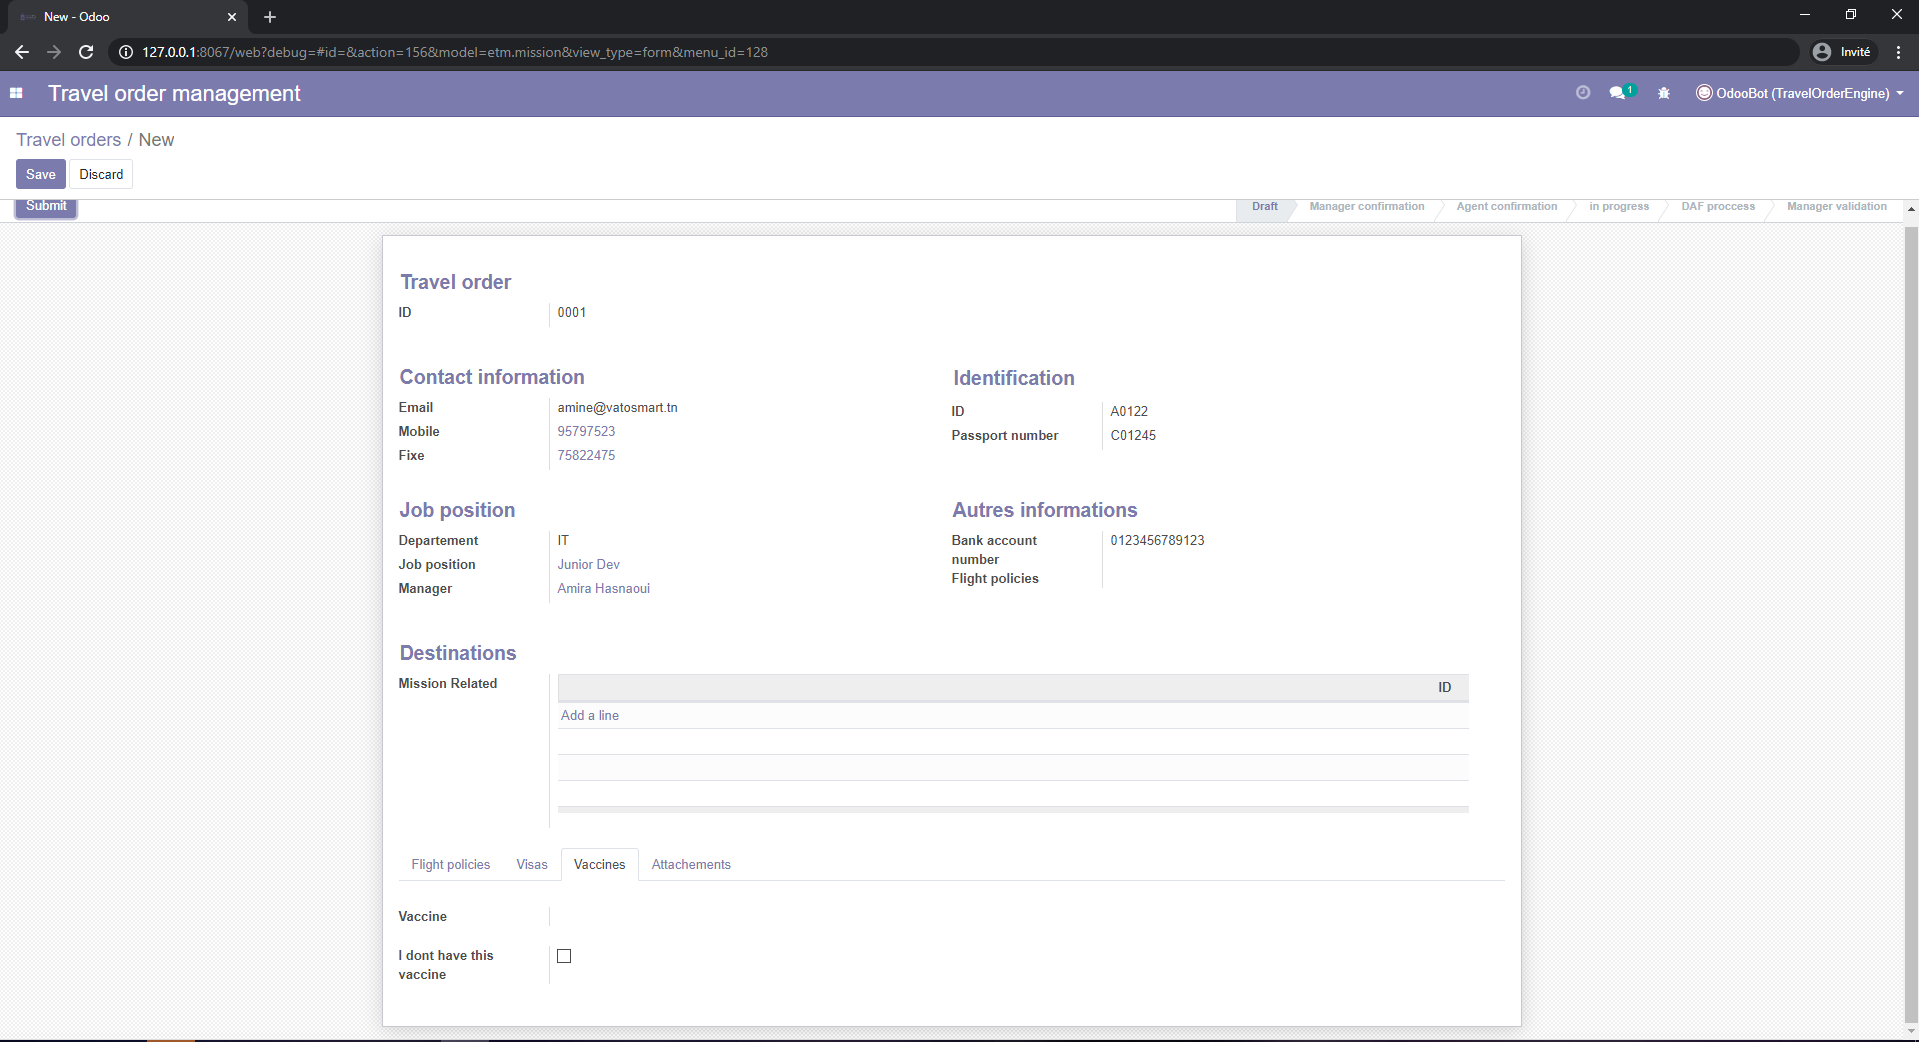
\includegraphics[scale=0.33]{img/c_mission_draft.png}
    \caption{travel order draft view}
    \label{fig:my_label}
\end{figure}

Clicking on the "Add a line" on the destinations list will open a pop-up window that contains a form with all needed information , This figure shows that form view.\\
Policies, Visas, Vaccines are not editable and are automatically generated based on the employee information and the destination country.
\begin{figure}[H]
    \centering
    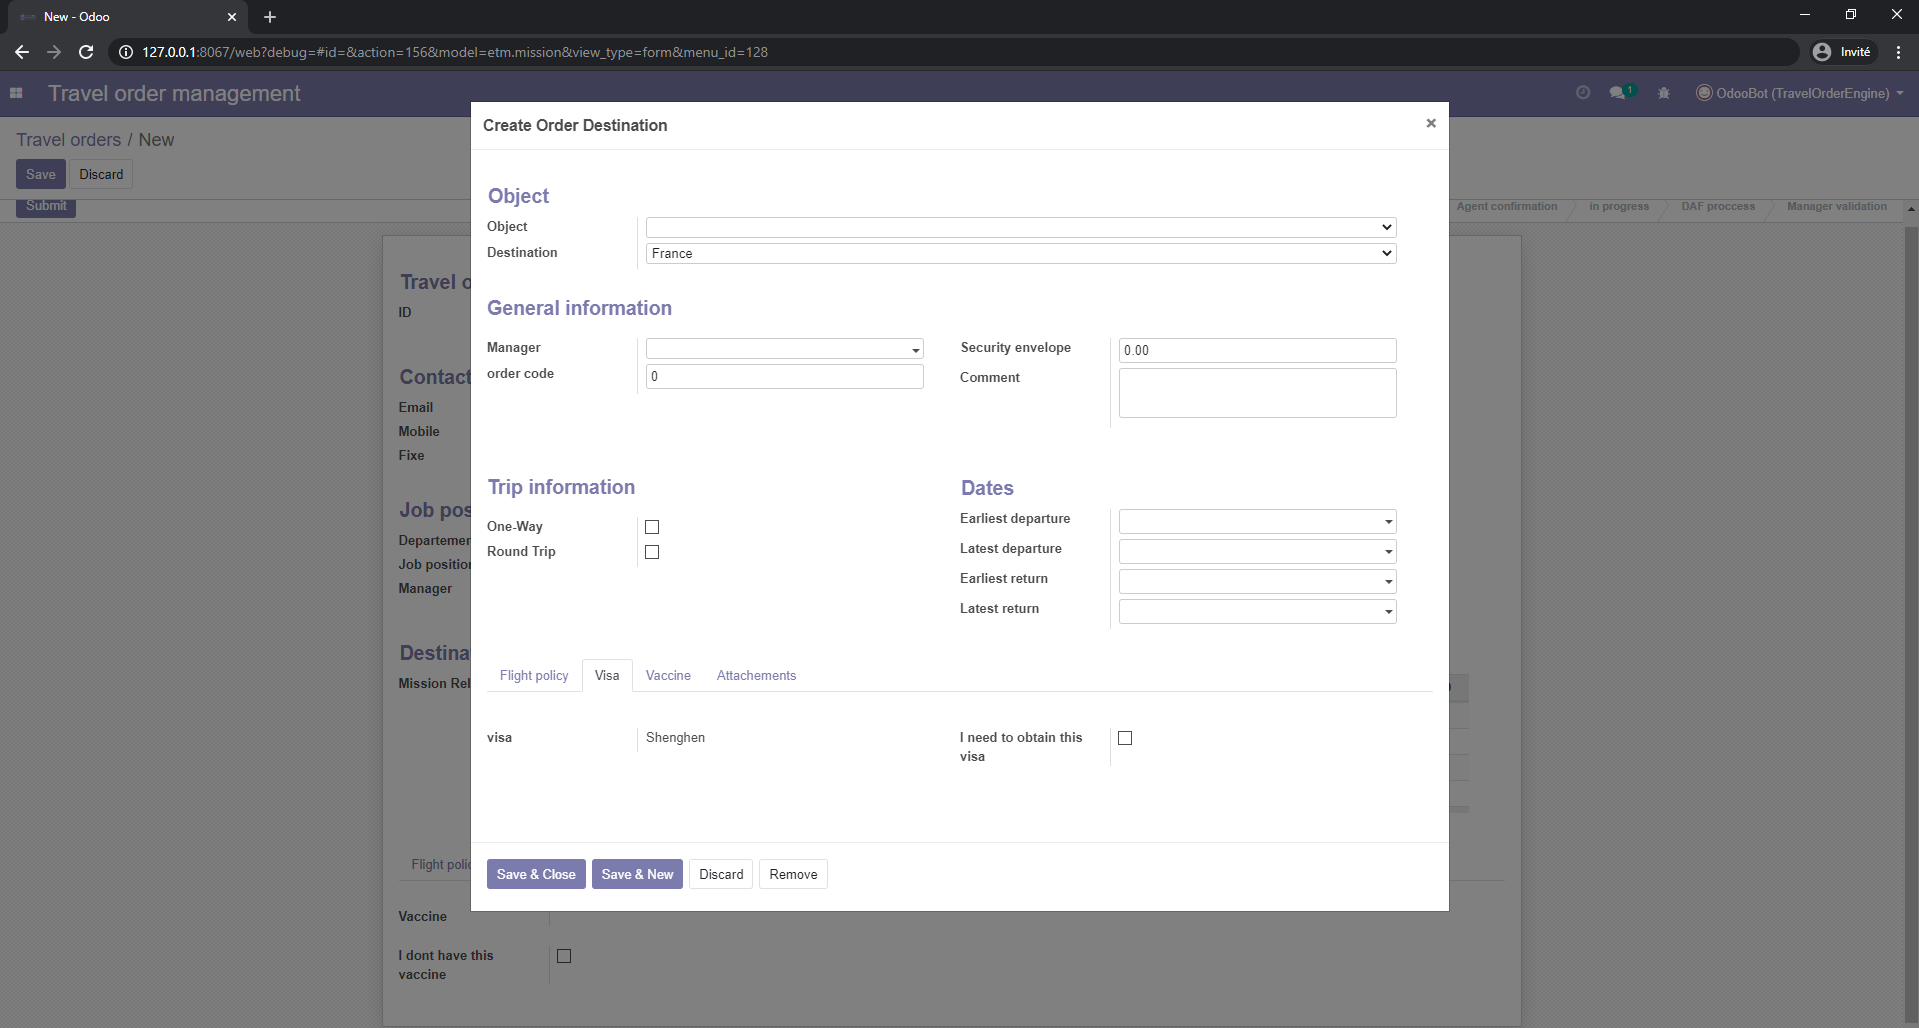
\includegraphics[scale=0.33]{img/c_destination_form.png}
    \caption{travel order destination form}
    \label{fig:my_label}
\end{figure}
The initial manager confirmation, the agent confirmation and the final manager validation are all basically the same static order view but with different workflow state and action buttons. during these phases the actor can only confirm or deny the order. In this figure we will show the manager confirmation
\begin{figure}[H]
    \centering
    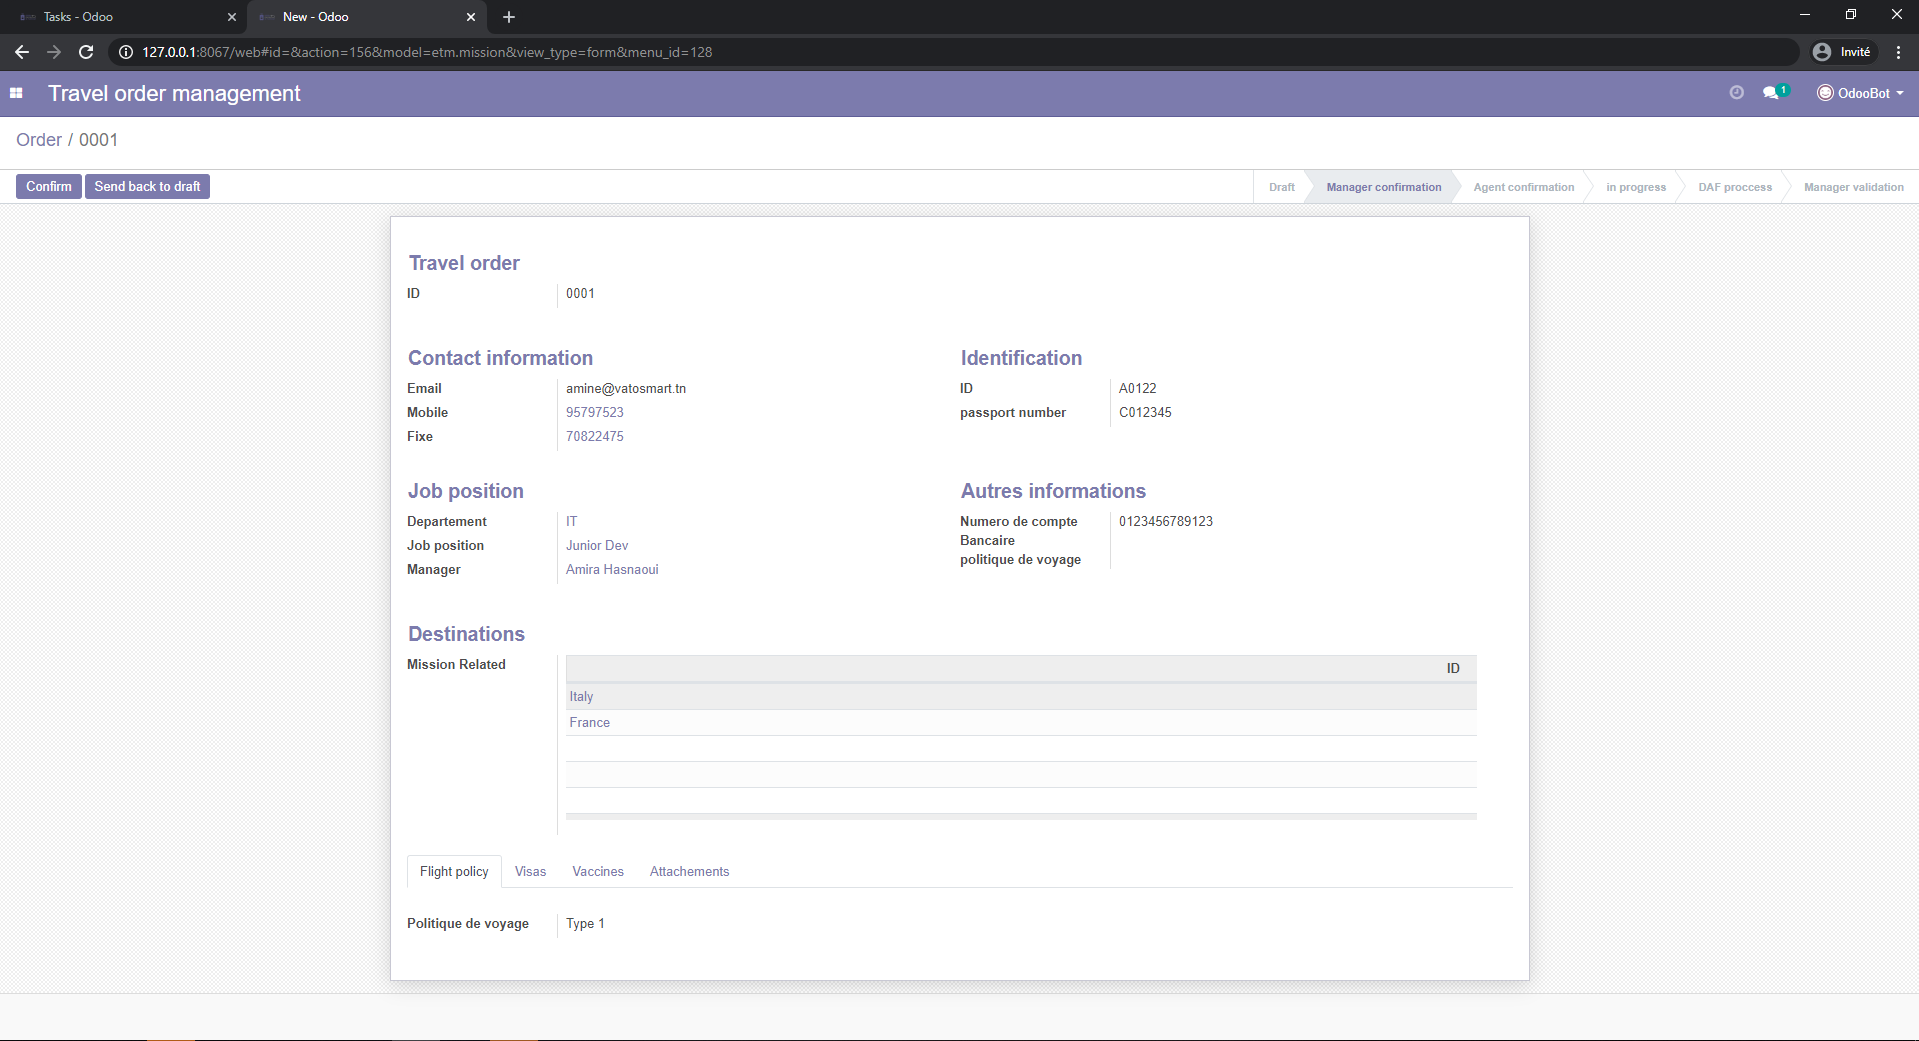
\includegraphics[scale=0.33]{img/c_manager_confirmation.png}
    \caption{Travel order confirmation view}
    \label{fig:my_label}
\end{figure}
In this last figure we will the agent dashboard , where agents can see all approved travel orders and change their status by drag-and-droping the order cards into the "in progress" and "Done" sections.

\begin{figure}[H]
    \centering
    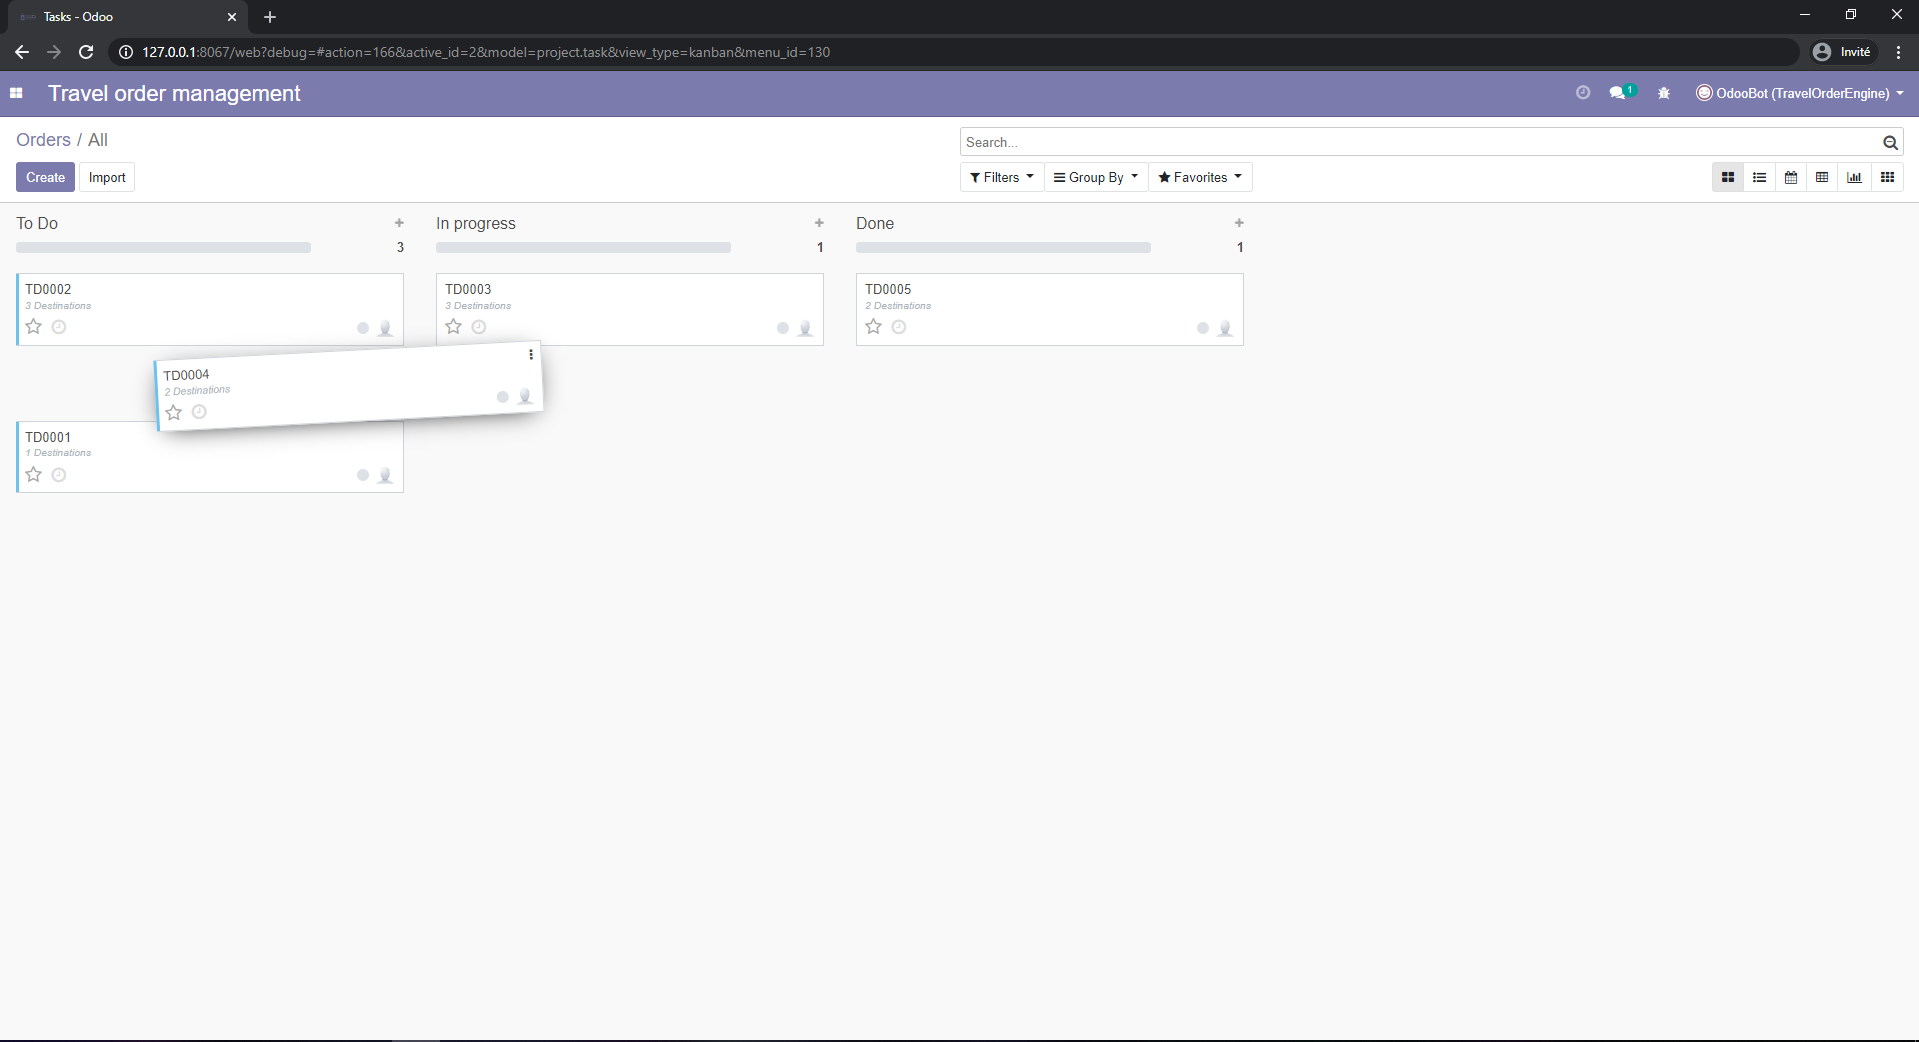
\includegraphics[scale=0.32]{img/c_agent_dash.png}
    \caption{Agent dashboard view}
    \label{fig:my_label}
\end{figure}






\section*{Conclusion}
  This sixth chapter summarized the work done during the third sprint of our project's life cycle, which was the design, development and implementation of a travel order management module. We started with the development of the Backlog sprint,then we started a design phase and we closed this chapter by exposing the interfaces of the developed module.
        \clearpage
        
        \section*{General conclusion}
Through this report, I presented the work I did during my internship with
VIPAY SARL. The objective of the internship was the design and implementation of an insturctor dashboard for the website study.tn.
\hfill \break
Regarding the approach, we first carried out a phase of analysing the existing tool. Second, we specified our application and it's major advantages compared to the existing solution. Thirdly, we proceeded to its modeling and design. Finally, we have implemented it.
\hfill \break
This was a good learning experience, it allowed me to discover the different
web programming techniques associated with React as well as discovering the world of e-learning.
        \clearpage
        
        % @author: Stoufa
		% the command `\nocite{*}` is mandatory to avoid the “no \citation commands” error
        % https://tex.stackexchange.com/questions/18045/problem-with-compiling-bibtex-no-citation-commands-error
        %\nocite{*}
        \printbibliography[heading=bibintoc]
        
   

    \backmatter
        
\thispagestyle{backcover}
\newgeometry{bottom=25mm,left=15mm,top=20mm,right=15mm}

\begin{changemargin}{3mm}{0cm}
    \begin{minipage}[c]{0.96\columnwidth}
        
        \selectlanguage{arabic}
        
        {\LARGE\textbf{ملخّص}}
        \vskip1mm
            \begingroup
                \small
                \@arabicAbstract
            \endgroup
        \vskip1mm
        {\textbf{كلمات مفاتيح : } 
            \begingroup
                \@arabicAbstractKeywords
            \endgroup
        }
        
        {\ifthenelse{\boolean{wantToTypeCompanyAddress}}
        {% IF TRUE
            \vskip5mm
        }{\vskip8mm}}
        
        \selectlanguage{french}
        
        {\LARGE\textbf{Résumé}}
        \vskip1mm
            \begingroup
                \large
                \@frenchAbstract
            \endgroup
        \vskip1mm
        {\textbf{Mots clés : }
            \begingroup
                \@frenchAbstractKeywords
            \endgroup
        }
        
        {\ifthenelse{\boolean{wantToTypeCompanyAddress}}
        {% IF TRUE
            \vskip5mm
        }{\vskip8mm}}
        
        \selectlanguage{english}
        {\LARGE\textbf{Abstract}}
        \vskip1mm
            \begingroup
                \large
                \@englishAbstract
            \endgroup
        \vskip1mm
        {\textbf{Keywords : }
            \begingroup
                \@englishAbstractKeywords
            \endgroup
        }
    \end{minipage}
    
\end{changemargin}
    
\end{document}